\documentclass[11pt]{article}
\usepackage[utf8]{inputenc}
\usepackage{amsthm}
\usepackage{amssymb}
\usepackage{fullpage}
\usepackage{epsfig}
\usepackage{enumitem}
\usepackage{amsmath}
\usepackage{amsfonts}
\usepackage[]{algorithm2e}
\usepackage{graphicx}
\usepackage[normalem]{ulem}
\usepackage{color}
\usepackage{subcaption}
\usepackage{multirow}
\usepackage{wrapfig}
\usepackage{titlesec}
\usepackage[margin=1.0in]{geometry}
\usepackage[font=small,labelfont=bf]{caption}
\graphicspath{figures/}

\DeclareMathOperator*{\argmax}{arg\,max}
\DeclareMathOperator*{\argmin}{arg\,min}


\title{\vspace{-2cm}Dynamic Stable Matching}
\author{Yunlin (Ilene) Lu\footnote{Equal Contribution} $\qquad$ Mathieu Tuli${}^*$ $\qquad$ Anqi (Joyce) Yang${}^*$}
% \date{April 2021}
\setlength{\parindent}{0pt}
\setlength{\parskip}{10pt}
\titlespacing*{\section}{0pt}{0.25\baselineskip}{0.25\baselineskip}
\titlespacing*{\subsection}{0pt}{0.25\baselineskip}{0.25\baselineskip}
\titlespacing*{\paragraph}{0pt}{0.25\baselineskip}{0.25\baselineskip}

\begin{document}
\maketitle

% \vspace{-10mm}
% \section{Introduction}
% \subfile{sec/intro}

% \section{Related Work}
% \subfile{sec/related}

% \section{Problem Formulation}
% \subfile{sec/problem}

% \section{Experiments}
% \subfile{sec/experiment}

% \section{Dicussion}
% \subfile{sec/discussion}

\vspace{-12mm}
\section{Introduction}
 
The Stable Matching (SM) problem is a classical problem in computational social choice that attempts to find a stable match between two equally sized opposing sets of agents, where each agent reports a vector of preferences over agents in the opposing set. In the traditional setting, preferences or rankings are static and the fundamental goal is to find a perfect, stable match: a match where each unique man and woman are paired such that no pair of man $m$ or woman $w$ prefer each other to their current match. In this work, we aim to investigate a variant of this stable matching problem, where agents' rankings are dynamic over time. Specifically, we investigate the more realistic scenario where agents have dynamic utility vectors over the set of opposing agents. Thus, these utility vectors may change at each time step, thus changing the underlying ranking of each agent over time.

Under this dynamic setting, we will investigate the use of various algorithms to analyze how consistency of matchings and social welfare change over time. Specifically, we investigate the following:
\begin{itemize}
    \item Men Preferred Deferred Acceptance (MPDA) under different dynamics of utilities. We will analyze how social welfare and consistency of matches varies as the agents' utilities are subject to various dynamics imposed by a Gaussian probability distribution
    \item
\end{itemize}
\section{Related Works}
\paragraph{Stable Matching}
In their 1962 paper~\cite{galeshapley1962}, Gale and Shapeley first proposed the classical stable matching problem and the corresponding
Gale-Shapeley algorithm, with two versions: the Men-Proposing Deferred Acceptance (MPDA) algorithm and the Women-Proposing Deferred Acceptance (MPDA) algorithm. Both versions are proven to generate a stable matching and terminate in $n^2$ moves and less~\cite{irving1989textbook}. MPDA is man-optimal where every women gets her worst possible partner, while WPDA is woman-optimal. To address the imbalance, Irving et al.~\cite{irving1987efficient} further proposed a sex-optimal stable matching algorithm that operates at $\mathcal{O}(n^4)$.

\paragraph{Stable Matching Variants}
There are many variants of the stable matching problem. The survey paper by Iwama and Miyazaki~\cite{iwama2008survey} provides a comprehensive overview of the popular variants, including the many-to-one matching (Hospitals/Residents Matching Problem), non-bipartite matching (Roommates Matching Problem), many-to-many matching, three-dimensional matching with three parties, and preferences with incomplete lists and/or ties. In addition, Anshelevich et al.~\cite{Anshelevich2013} extend preference profile with numerical utilities to analyze the overall social welfare of stable matching. We share the same notion of numerical utilities when evaluating social welfare as~\cite{Anshelevich2013}, but none of the existing settings consider the dimension of time, so our setting remains novel.

\section{Problem Formulation}
% \begin{itemize}
%     \item 1.5 - 2 pages
%     \item Formulation for the set-up with utilities, excitement and dynamics
%     \item Metrics
%     \begin{itemize}
%         \item Stability
%         \item Social Welfare
%         \item Consistency
%         \item Explore social welfare vs. stability
%     \end{itemize}
% \end{itemize}
In this section, we formally describe the dynamic stable matching setting, followed by several desirable properties that a matching should have.
\subsection{Problem Setting}
In the classical stable matching problem setting, there are $N$ men and $N$ women where each man $m_i$ has a strict preference ranking $\overrightarrow{\succ}_{m_i}$ for the women and vice versa, and the goal is to find a perfect and stable matching $M$ such that no pair of man $m$ and woman $w$ prefer each other to their current matches. In this project, we study a variant of the stable matching problem with the modification that each agent's preference is induced by underlying numerical utilities, and that the utilities may change over time, prompting a need to re-match the agents for stability.

More formally, in our \textit{dynamic} stable matching setting, there are again $N$ men and $N$ women. Each man $m_i$ is associated with an underlying numerical utility vector $u_i \in \mathbb{R}^n$ satisfying $w_{j_1} \succ_{m_i} w_{j_2} \Leftrightarrow u_i(w_{j_1}) > u_i(w_{j_2})$ for every pair of women $(w_{j_1}, w_{j_2})$. Similarly, each women $w_j$ is associated with a utility vector $v_j \in \mathbb{R}^n$ consistent with her preferences for the group of men. The utilities are normalized, i.e., $\sum_{j=1}^N{u_i(w_j)} = 1$ for every $m_i$, and $\sum_{i=1}^N{v_j(m_i)} = 1$ for every $w_j$.

In addition, each agent also has an excitement vector for each viable candidate. Formally, each man $m_i$ has an excitement vector $x_i \in \mathbb{R}^n$ where each $x_i(w_j)$ denotes the excitement man $m_i$ has for woman $w_j$. Similarly, each woman $w_j$ has an excitement vector $y_j \in \mathbb{R}^n$ representing her excitement towards each man. All excitement vectors are non-negative.

Furthermore, we add a time dimension to the problem. For simplicity, instead of working with the infinite continuous time domain, we define a finite set of discrete times $t \in \{1, \ldots, T\}$, and each person's utility vector will change according to the excitement and and current matching over time according to the following rule. At each time step $t$, with everyone's utilities $\overrightarrow{u}^{t}$ and $\overrightarrow{v}^{t}$ and the computed matching $M^t$, we derive the updated utilities $\overrightarrow{u}^{t+1}$ and $\overrightarrow{v}^{t+1}$ for each man $m_i$ and woman $w_j$ as follows:
    \begin{align*}
        & u^{t+1}_i(w_j) = \begin{cases} u^t_i(w_j) * (1 + x_i(w_j)) &\text{if $M^t(m_i) \neq w_j$} \\ u^t_i(w_j) * (1 - x_i(w_j)) &\text{if $M^t(m_i) = w_j$} \end{cases},\\
        & v^{t+1}_j(m_i) = \begin{cases} v^t_j(m_i) * (1 + y_j(m_i)) &\text{if $M^t(w_j) \neq m_i$} \\ v^t_j(m_i) * (1 - y_j(m_i)) &\text{if $M^t(w_j) = m_i$} \end{cases}.
    \end{align*}
In other words, the matched couple have decreased utilities towards each other and increased utilities for all other candidates. As a result, we will need to re-run the matching algorithm to generate a new matching $M^{t+1}$. Depending on the updated utilities $\overrightarrow{u}^{t+1}$ and $\overrightarrow{v}^{t+1}$, the couples from $M^t$ may not stay together in the new matching $M^{t+1}$.


\subsection{Metrics}
We design this new setting with inspirations from relationships in the real world, where people can divorce and enter new marriages over time due to changed utilities towards each other. We evaluate the matches with the following metrics.
\paragraph{Stability} We measure the instability of a series of matches $(M^1, \ldots, M^T)$ with the mean number of blocking pairs, i.e.,
\begin{equation}
    \mbox{instability}(M^1, \ldots, M^T) = \frac{1}{T}\sum_{t=1}^T{\frac{\sigma(M^t)}{N}},
\end{equation}
where $\sigma(M^t)$ is the number of blocking pairs in $M^t$.
\paragraph{Social Welfare} We define the social welfare of a series of matches as the mean utilities each agent derives from the matching:
\begin{equation}
    \mbox{sw}(M^1, \ldots, M^T) = \frac{1}{T}\sum_{t=1}^T{\frac{1}{2N}{\sum_{(m_i, w_j)\in M^t}{u_i(w_j) + v_j(m_i)}}}.
\end{equation}
\paragraph{Consistency} We also would like to encourage the couples to stay together over time. We define the consistency of a series of matches to be:
\begin{equation}
    \mbox{consistency}(M^1, \ldots, M^T) = \frac{1}{T-1}\sum_{t=1}^{T-1}{|\{(m, w): (m, w) \in M^t \wedge (m, w) \in M^{t+1}\}|}.
\end{equation}
\paragraph{Stability vs. Social Welfare} Note that stability and social welfare are both metrics that take into account of the preference profiles/utilities of the agents, but one does not necessarily imply the other. It is easy to show that a max social welfare matching $M$ is not necessarily stable, and a stable matching might not maximize social welfare.

Max social welfare $\nRightarrow$ stability: Consider two men and two women where $m_1$ has utility 1 towards $w_1$ and utility 0 towards $w_2$, $m_2$ has utility 0.6 towards $w_1$ and 0.4 towards $w_2$, $w_1$ has utility 0.4 towards $m_1$ and 0.6 towards $m_2$, and $w_2$ has utility 0 towards $m_1$ and 1 towards $m_2$. In this setting, $M = \{(w_1, m_1), (w_2, m_2)\}$ is the matching that maximizes social welfare, but it is not stable as $m_2$ and $w_1$ both prefer each other more than the matched partner.

Stability $\nRightarrow$ max social welfare: In the setting above, $M' = \{(m_1, w_2), (m_2, w_1)\}$ is a stable pair, but it achieves less social welfare than $M$.

Our goal is to empirically evaluate a few matching algorithms in different settings of utility and excitement initialization, and identify algorithms that can produce matches with high stability, high social welfare and high consistency.
\section{Experiments}
We first investigate the effect of different dynamics settings have on the performance. We then evaluate a few different matching algorithms to study the trade-off between stability, social welfare and consistency.
\subsection{Experimental Set-up}
% 0.5-1 page
% \begin{itemize}
%     \item Algorithms we are evaluating
%     \begin{itemize}
%         \item MPDA, WPDA
%         \item Probabilistic-based that always selects the best stable matching with a probability
%         \item Probabilistic-based that always selects the best matching with a probability
%         \item [Stretch] Deterministic algorithm that always selects the best sw with a consistency above a certain threshold
%     \end{itemize}
%     \item Dynamics
%     \item Number of agents, time steps, etc.
%     \item Evaluation set-up
% \end{itemize}
\paragraph{Dynamics Setting} For each agent, we independently initialize each utility value by sampling from a normal distribution $\mathcal{N}(\mu_u, \sigma_u^2)$ with scalar mean $\mu_u \in \mathbb{R}$ and variance $\sigma_u^2 \in \mathbb{R}$. For each utility value $x$, we clip it at 0 with $x \leftarrow \max(x, 0)$ to ensure it is non-negative. We further normalize the utilities such that each agent's utility vector has a total sum of 1. In addition, we independently sample each agent's excitement from a normal distribution $\mathcal{N}(\mu_e, \sigma_e^2)$. We clip the excitements at 0 such that the values are non-negative.

\paragraph{Algorithms} We implement both the Men Proposing Deferred Acceptance (MPDA) and the Women Proposing Deferred Acceptance (WPDA) algorithms~\cite{galeshapley1962}, which are guaranteed to return a stable matching. In addition, we implement a family of deterministic algorithms (Det) and a family of probabilistic algorithms (Prob, Prob-Stable), described as follows.

\textit{\textbf{Det}}: This is a family of algorithms parameterized by $c \in [0, 1]$ and returns a perfect matching with $$M^{t+1} = \argmax_{\mbox{consistency}(M^t, M) \ge c}{\mbox{sw}(M)}.$$
% In other words, the generated matching $M^{t+1}$ is the matching maximizing the social welfare subjected to the condition that the consistency is at least $c$ compared to the most recent match.
Solving for $M^{t+1}$ requires enumerating through all possible matching with consistency at least $c$. For computational efficiency, we perform the following approximation: we first identify and fix $N * c$ couples in $M^t$ that have the highest social welfare according to the updated utilities $\overrightarrow{u}^{t+1}$ and $\overrightarrow{v}^{t+1}$, and re-match the rest with the Hungarian Algorithm~\cite{Kuhn55thehungarian,Kuhn56thehungarian,Munkres1957Assignment} over the remaining men and women to obtain the maximum weight perfect bipartite matching, where the weight between a man node $m_i$ and a woman node $w_j$ in the bipartite graph is $u_i^{t+1}(w_j) + v_j^{t+1}(m_i)$. The generated new matching, which keeps at least the same $N*c$ couples from before, thus has consistency of at least $c$ and reasonably large social welfare.

\textit{\textbf{Prob}}: This family of algorithms is parameterized by a probability value $p$ and finds a matching as follows:
$$M^{t+1} = \begin{cases} \argmax_M{\mbox{sw}(M)} &\text{with probability $1-p$}\\ M^t &\text{with probability $p$}\end{cases}.$$
As a result, the expected consistency is at least $p$. We find $\argmax_M{\mbox{sw}(M)}$ by running the Hungarian algorithm on the full bipartite graph.

\textit{\textbf{Prob-Stable}} A variant of the probabilistic algorithm is to always return a \textit{stable} matching that has the maximum possible social welfare with probability $1-p$. However, in the case where we keep the previous matching $M^t$, since $M^t$ might not be stable with the updated utilities, Prob-Stable is not guaranteed to have stable matches all the time. One side note that it is infeasible to have the \textit{Det-Stable} variant, as stable matching might not exist for high consistency thresholds.


\subsection{Results and Analysis}
\begin{figure}
    \centering
    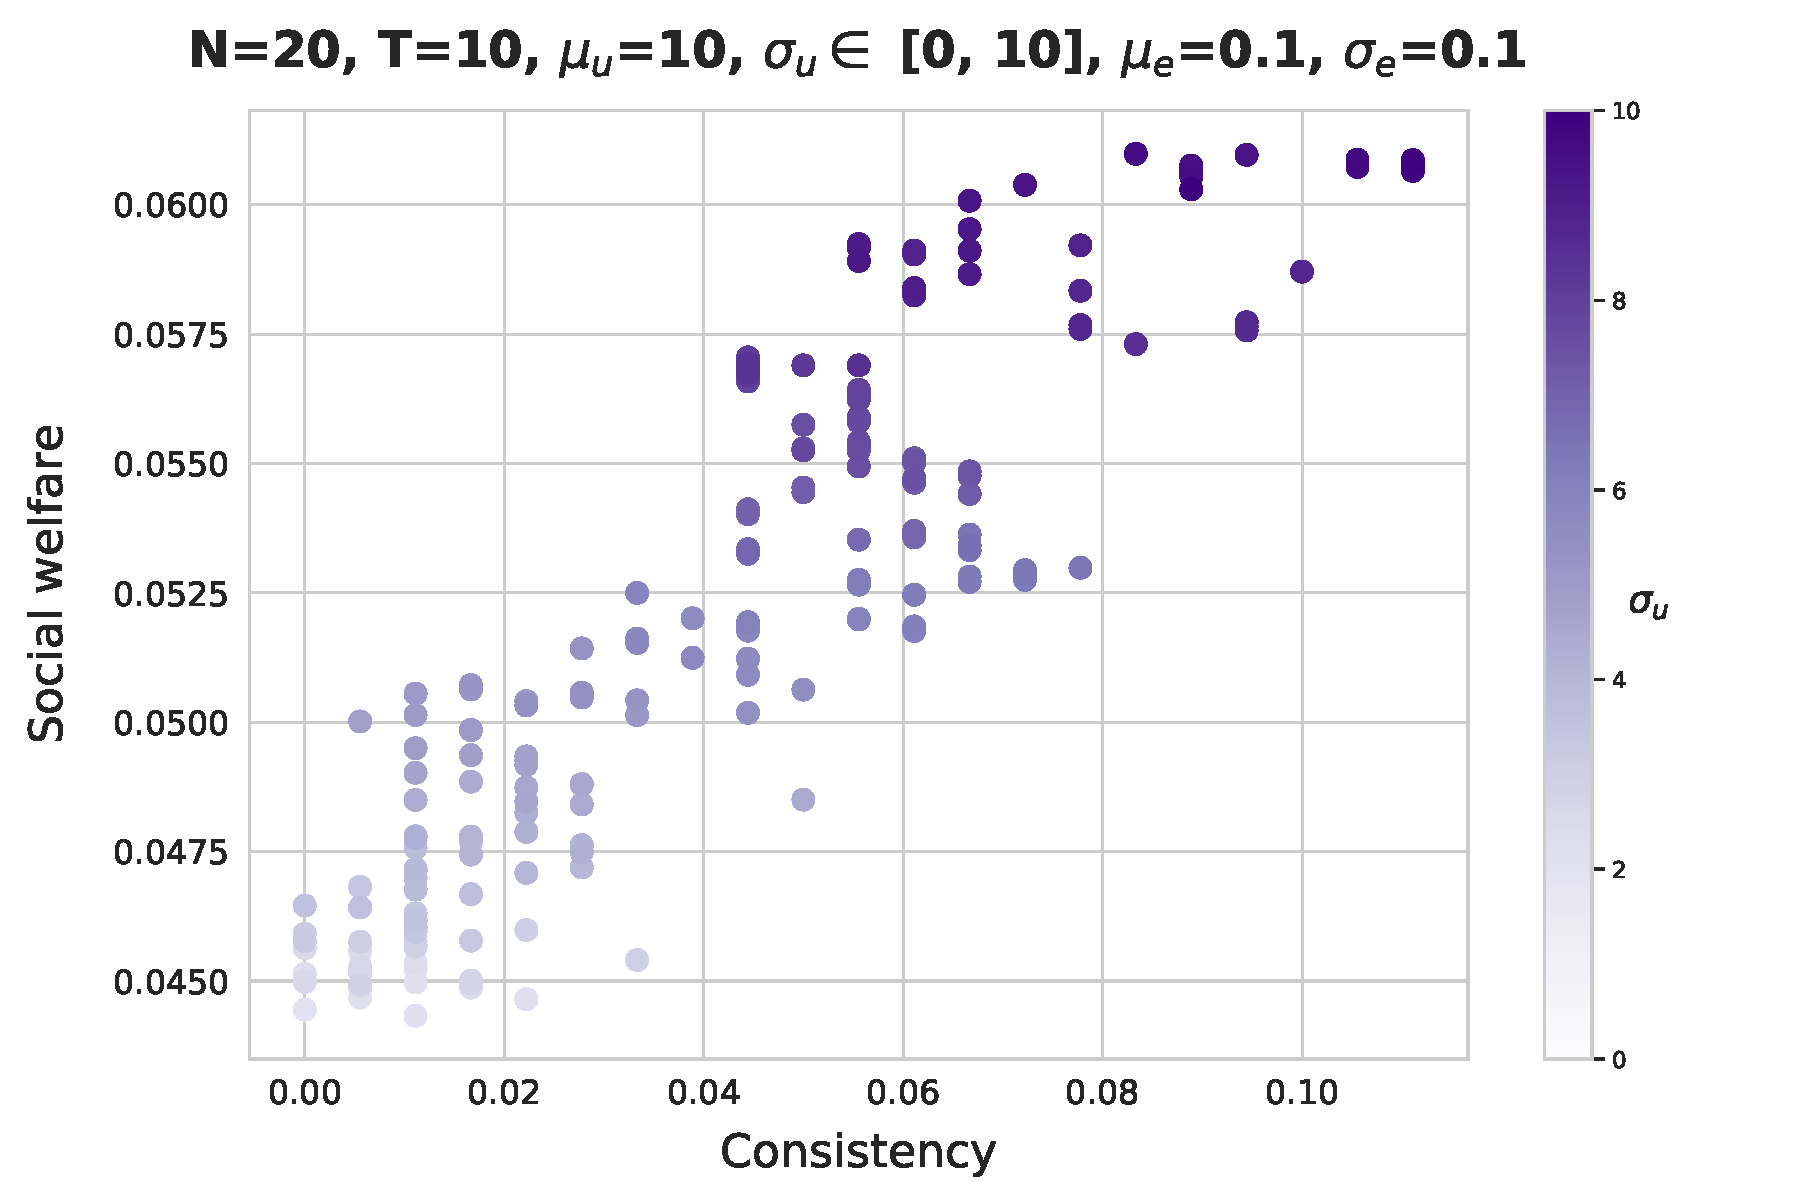
\includegraphics[width=0.32\linewidth]{figures/mpda_dynamics_initliazation.pdf}
    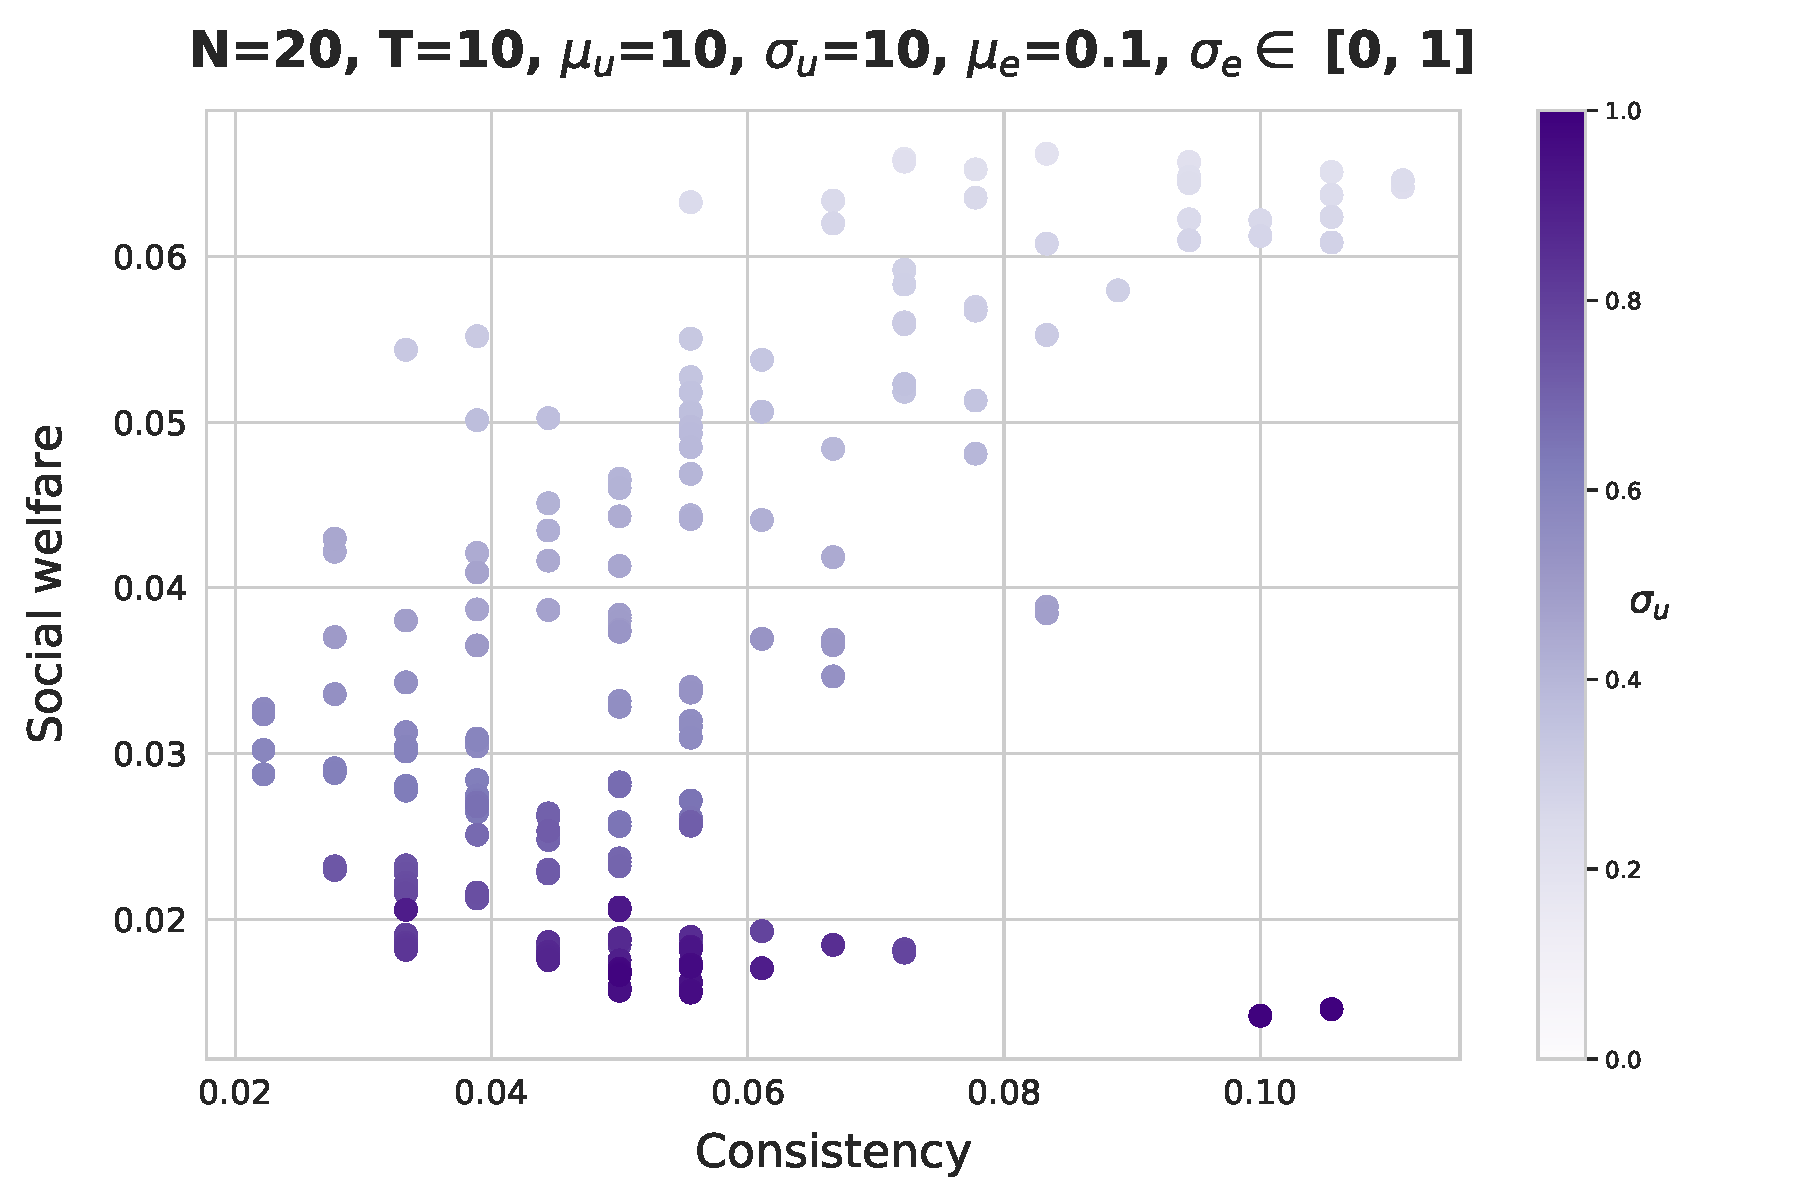
\includegraphics[width=0.32\linewidth]{figures/mpda_dynamics_excitement_std.pdf}
    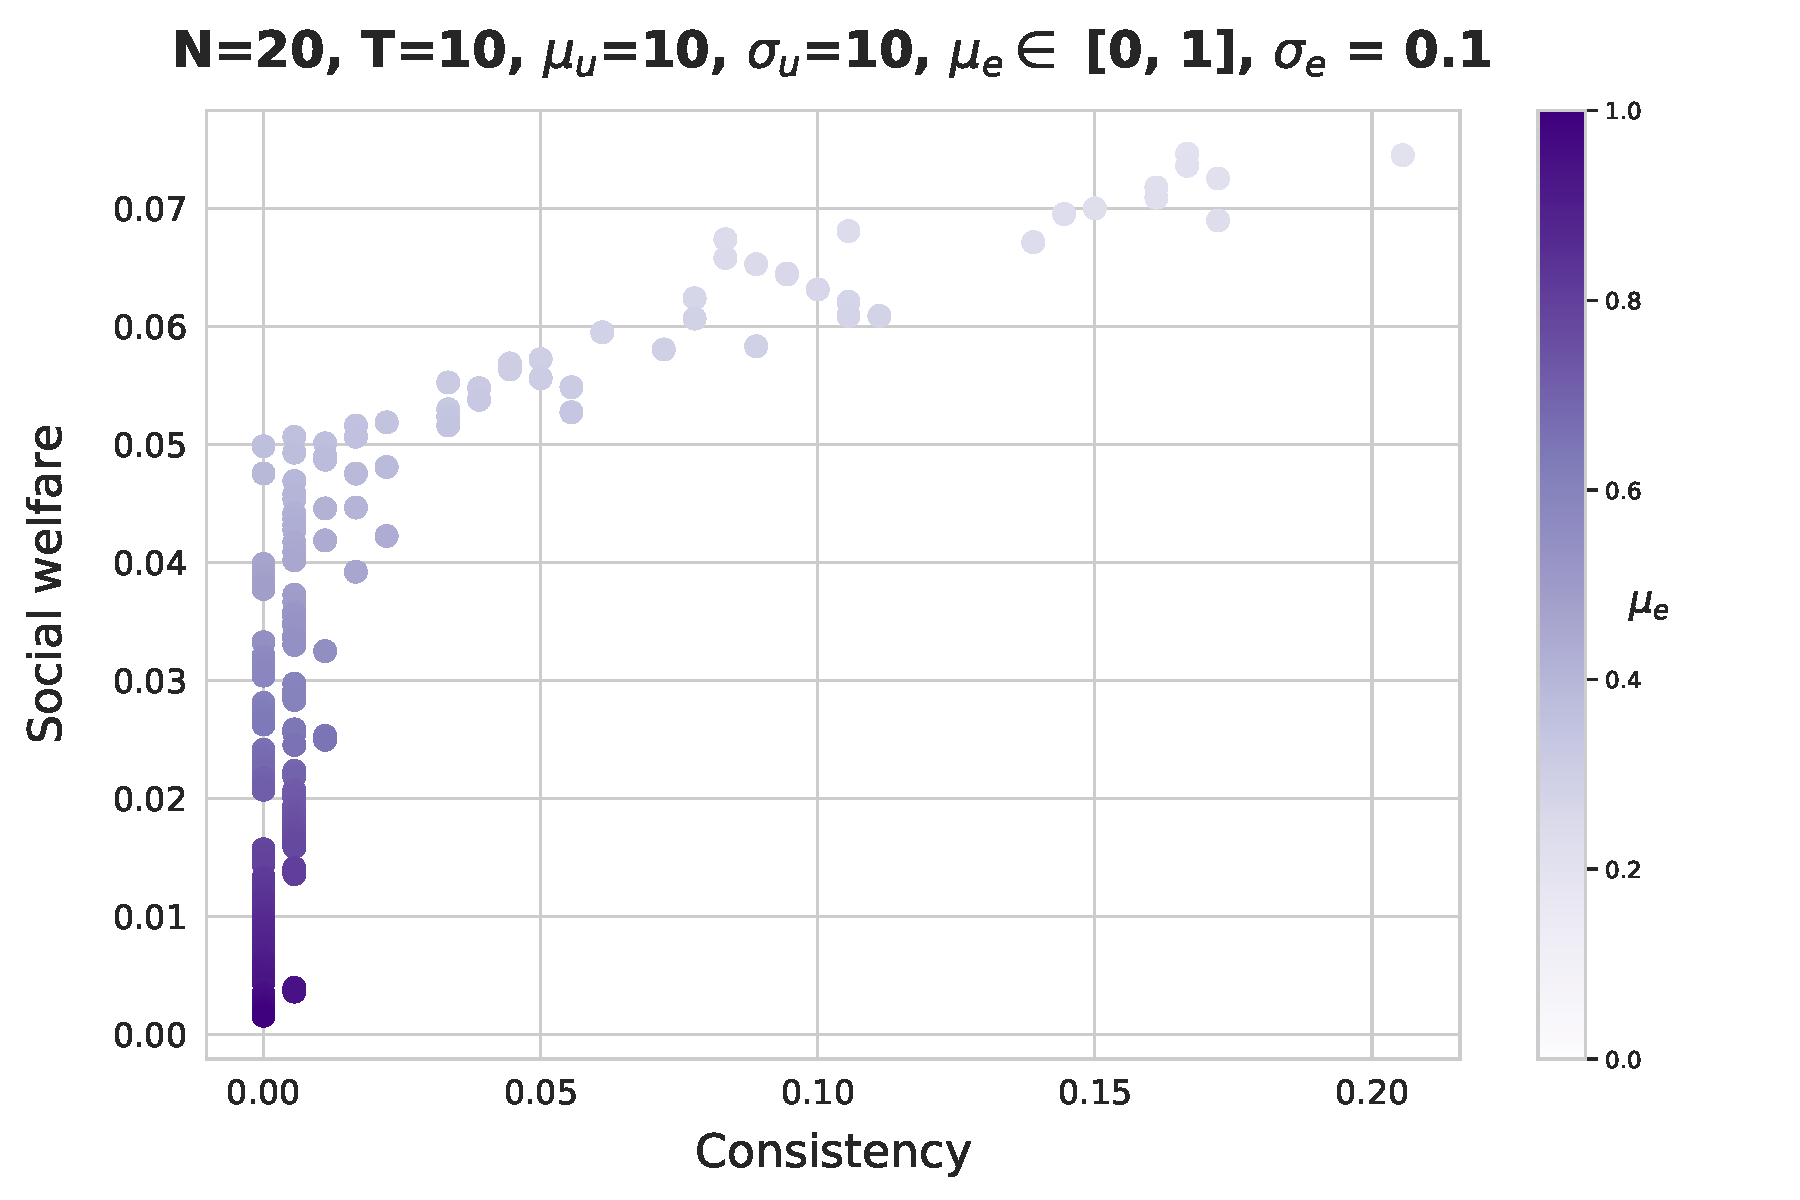
\includegraphics[width=0.32\linewidth]{figures/mpda_dynamics_excitement_mean.pdf}
     \caption{Mean social welfare vs. consistency for MPDA applied in various settings with 20 men/women and 10 time steps. (Left) Fixed excitement with varying utilities initialization (fixed mean). (Middle) Fixed utilities initialization but varying excitement (fixed mean) (b) fixed initialization varying excitement (fixed mean). (Right) Fixed utilities initialization but varying excitement (fixed variance).}
    \label{fig:mpda_dynamics}
\end{figure}
% \begin{figure}
%     \centering
%         \begin{subfigure}[b]{0.49\textwidth}
%          \centering
%          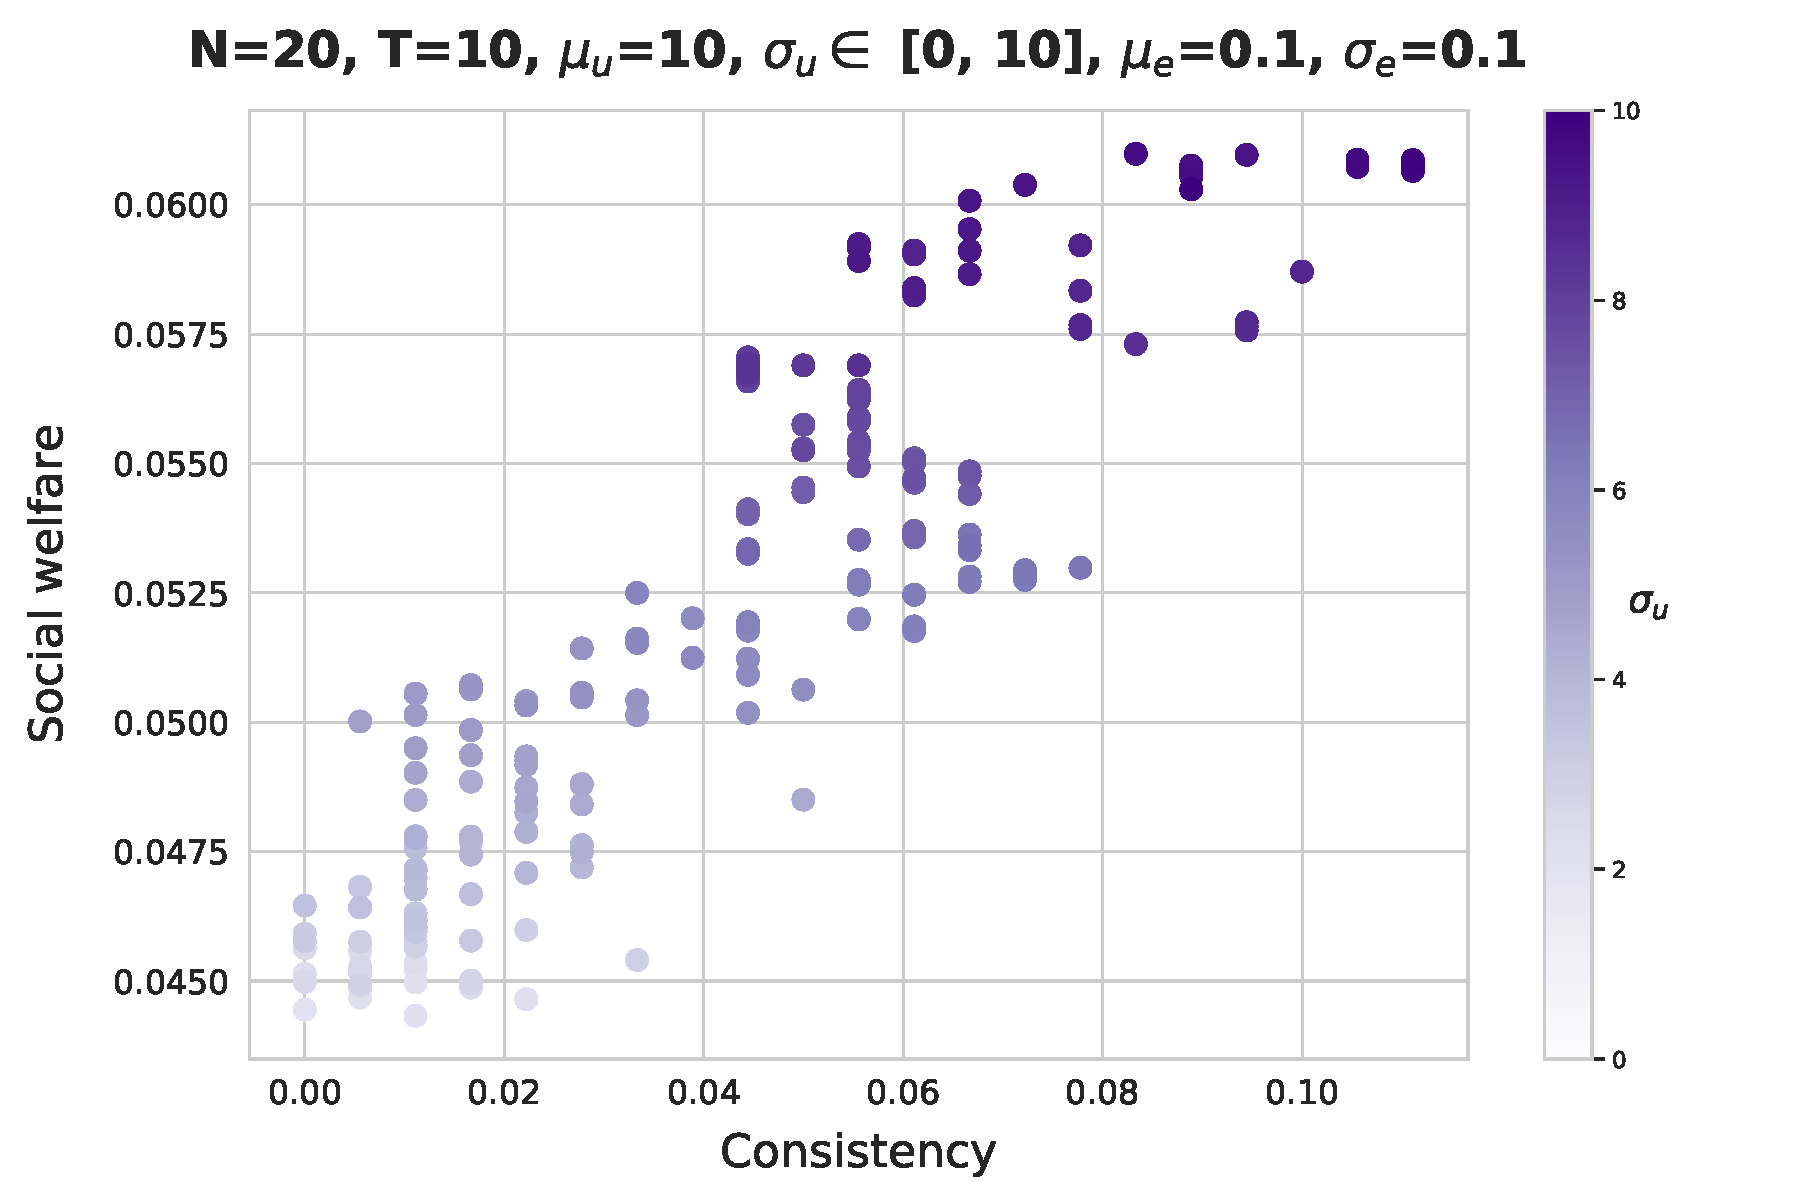
\includegraphics[width=\textwidth]{figures/mpda_dynamics_initliazation.pdf}
%          \caption{Dynamic Initialization}
%          \label{fig:init}
%         \end{subfigure}
%          \begin{subfigure}[b]{0.49\textwidth}
%          \centering
%          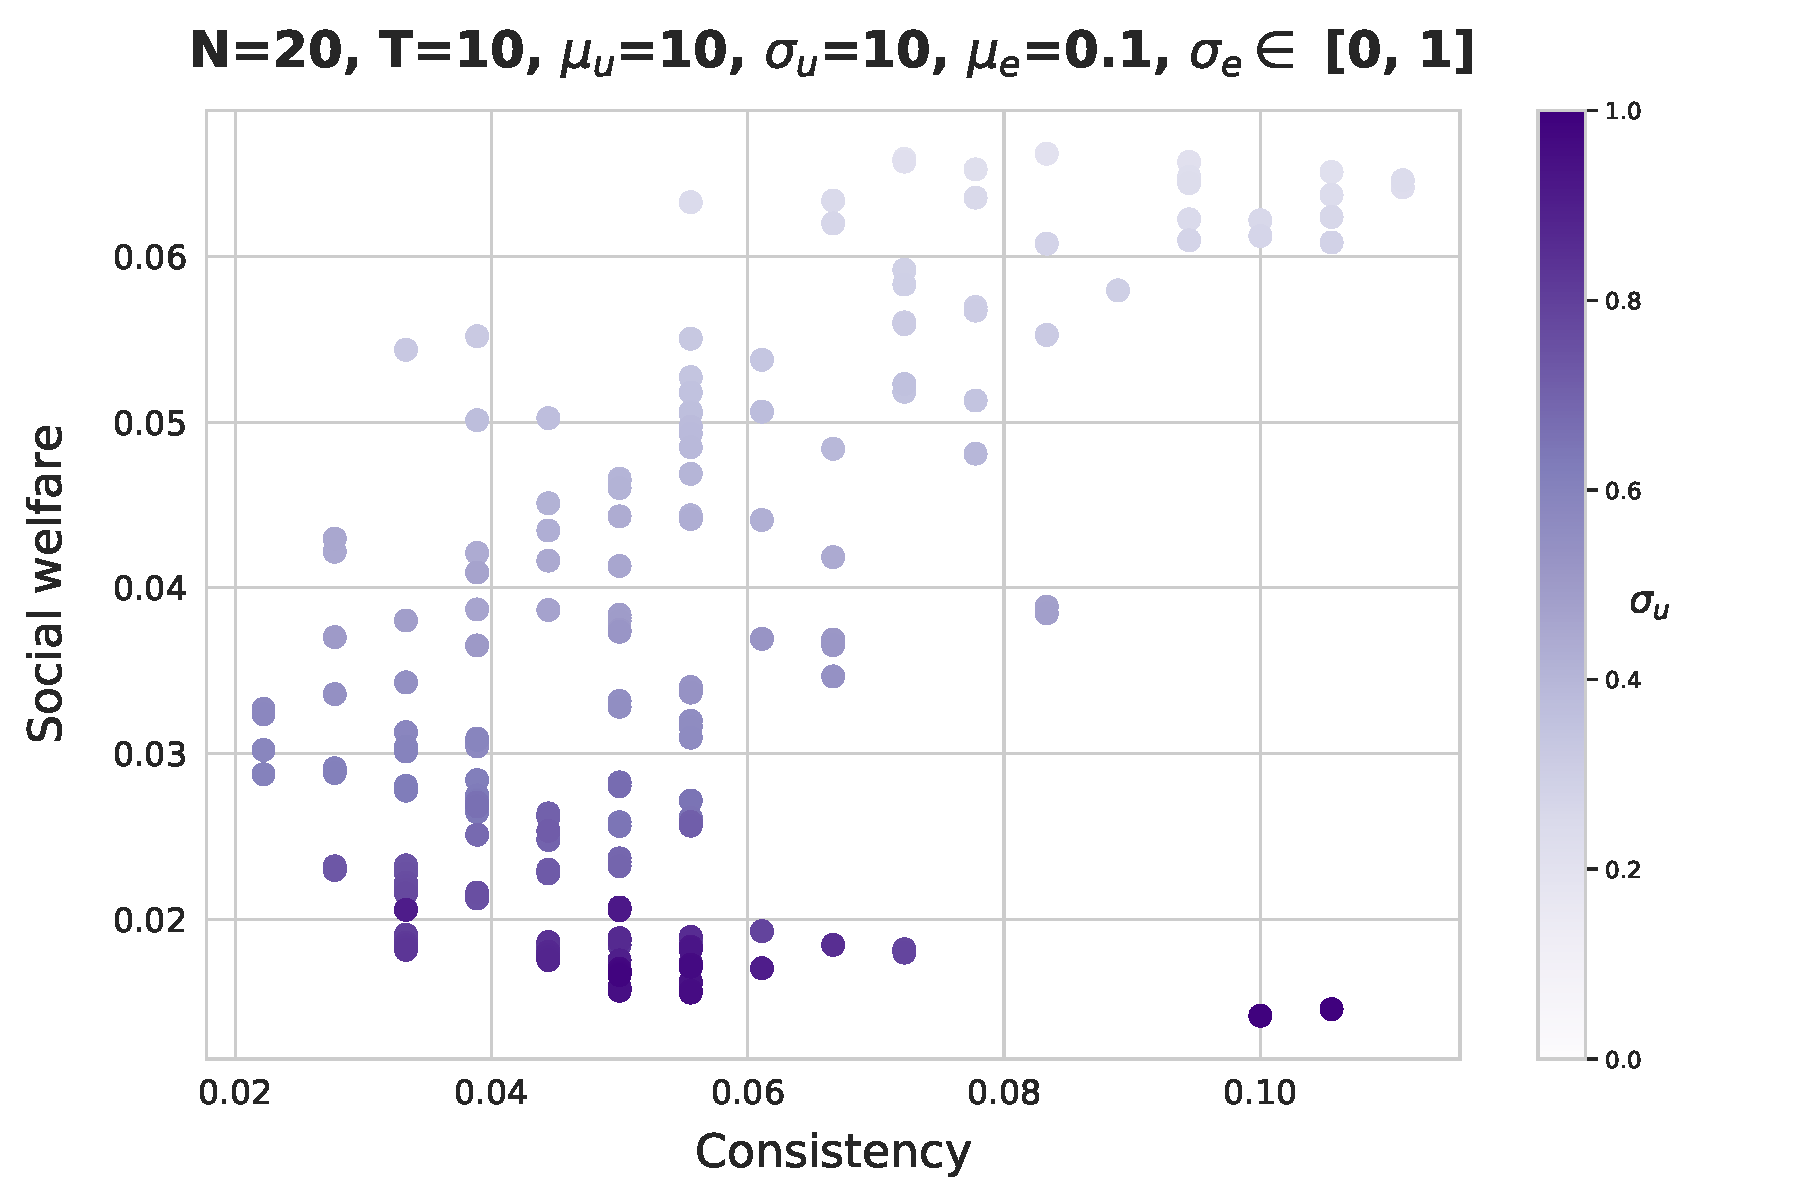
\includegraphics[width=\textwidth]{figures/mpda_dynamics_excitement_std.pdf}
%          \caption{Dynamic Excitement}
%          \label{fig:excite_std}
%      \end{subfigure}
%          \begin{subfigure}[b]{0.49\textwidth}
%          \centering
%          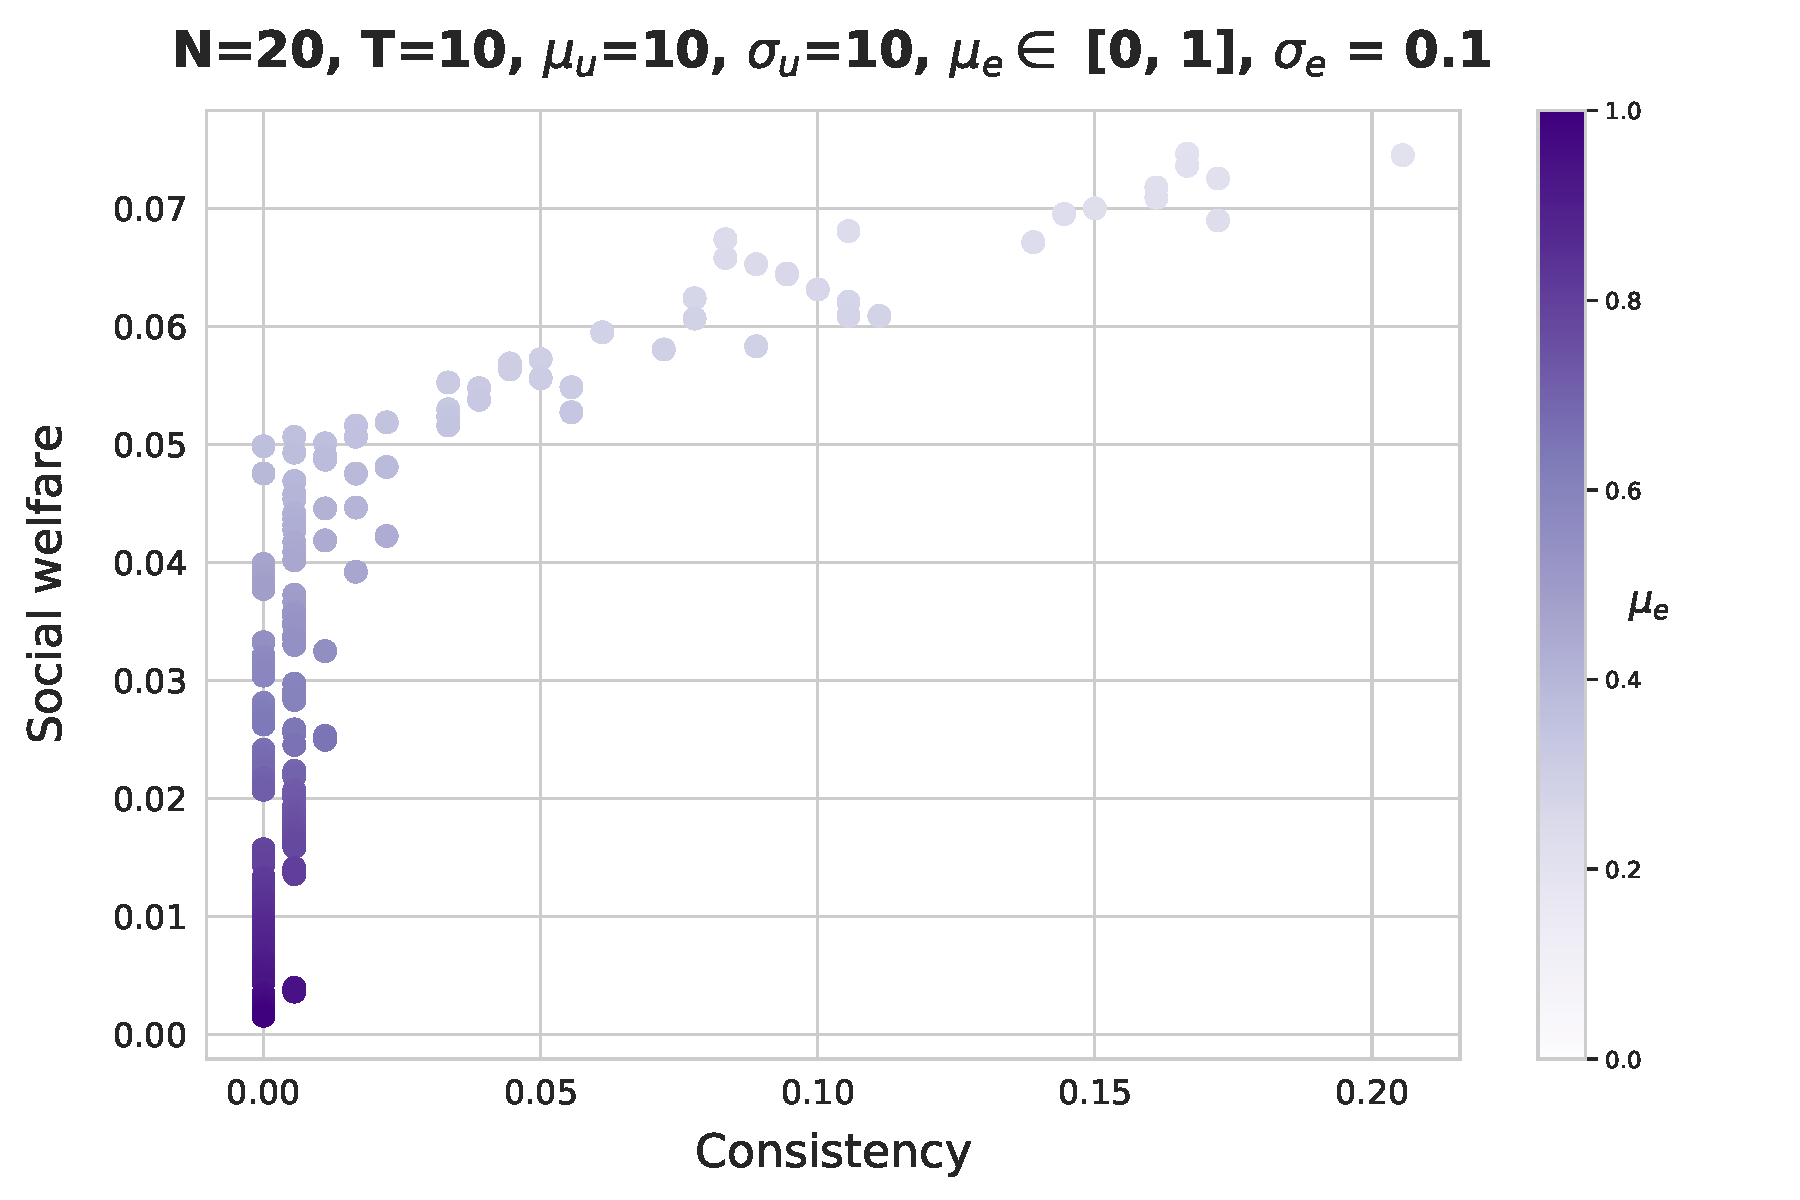
\includegraphics[width=\textwidth]{figures/mpda_dynamics_excitement_mean.pdf}
%          \caption{Dynamic Excitement}
%          \label{fig:excite_mean}
%      \end{subfigure}
%      \caption{Mean social welfare vs. consistency for MPDA applied to two dyanmic scenarios; (a) fixed excitement; (b) fixed initialization varying excitement (fixed mean); (c) fized initialization with varying excitement (fixed standard deviation).}
%     \label{fig:mpda_dynamics}
% \end{figure}

\paragraph{Dynamics} We first perform an ablation study with various utilities and excitement initializations. We run MPDA in a few dynamics settings with varying $\sigma_u$, $\mu_e$ and $\sigma_e$. Fig.~\ref{fig:mpda_dynamics} illustrates the results. Note that $\mu_u$ has little significant since the utilities are normalized, hence we did not experiment with varying $\mu_u$. The results show that with a larger $\sigma_u$ leads to both higher social welfare and consistency, most likely due to the fact that agents start out more loyal to their top choices and therefore it takes longer for the preference profile to shift. In addition, larger $\mu_e$ and $\sigma_e$ result in more dynamical changes to the utilities, which generally causes smaller social welfare and consistency.

\begin{figure}
    \centering
    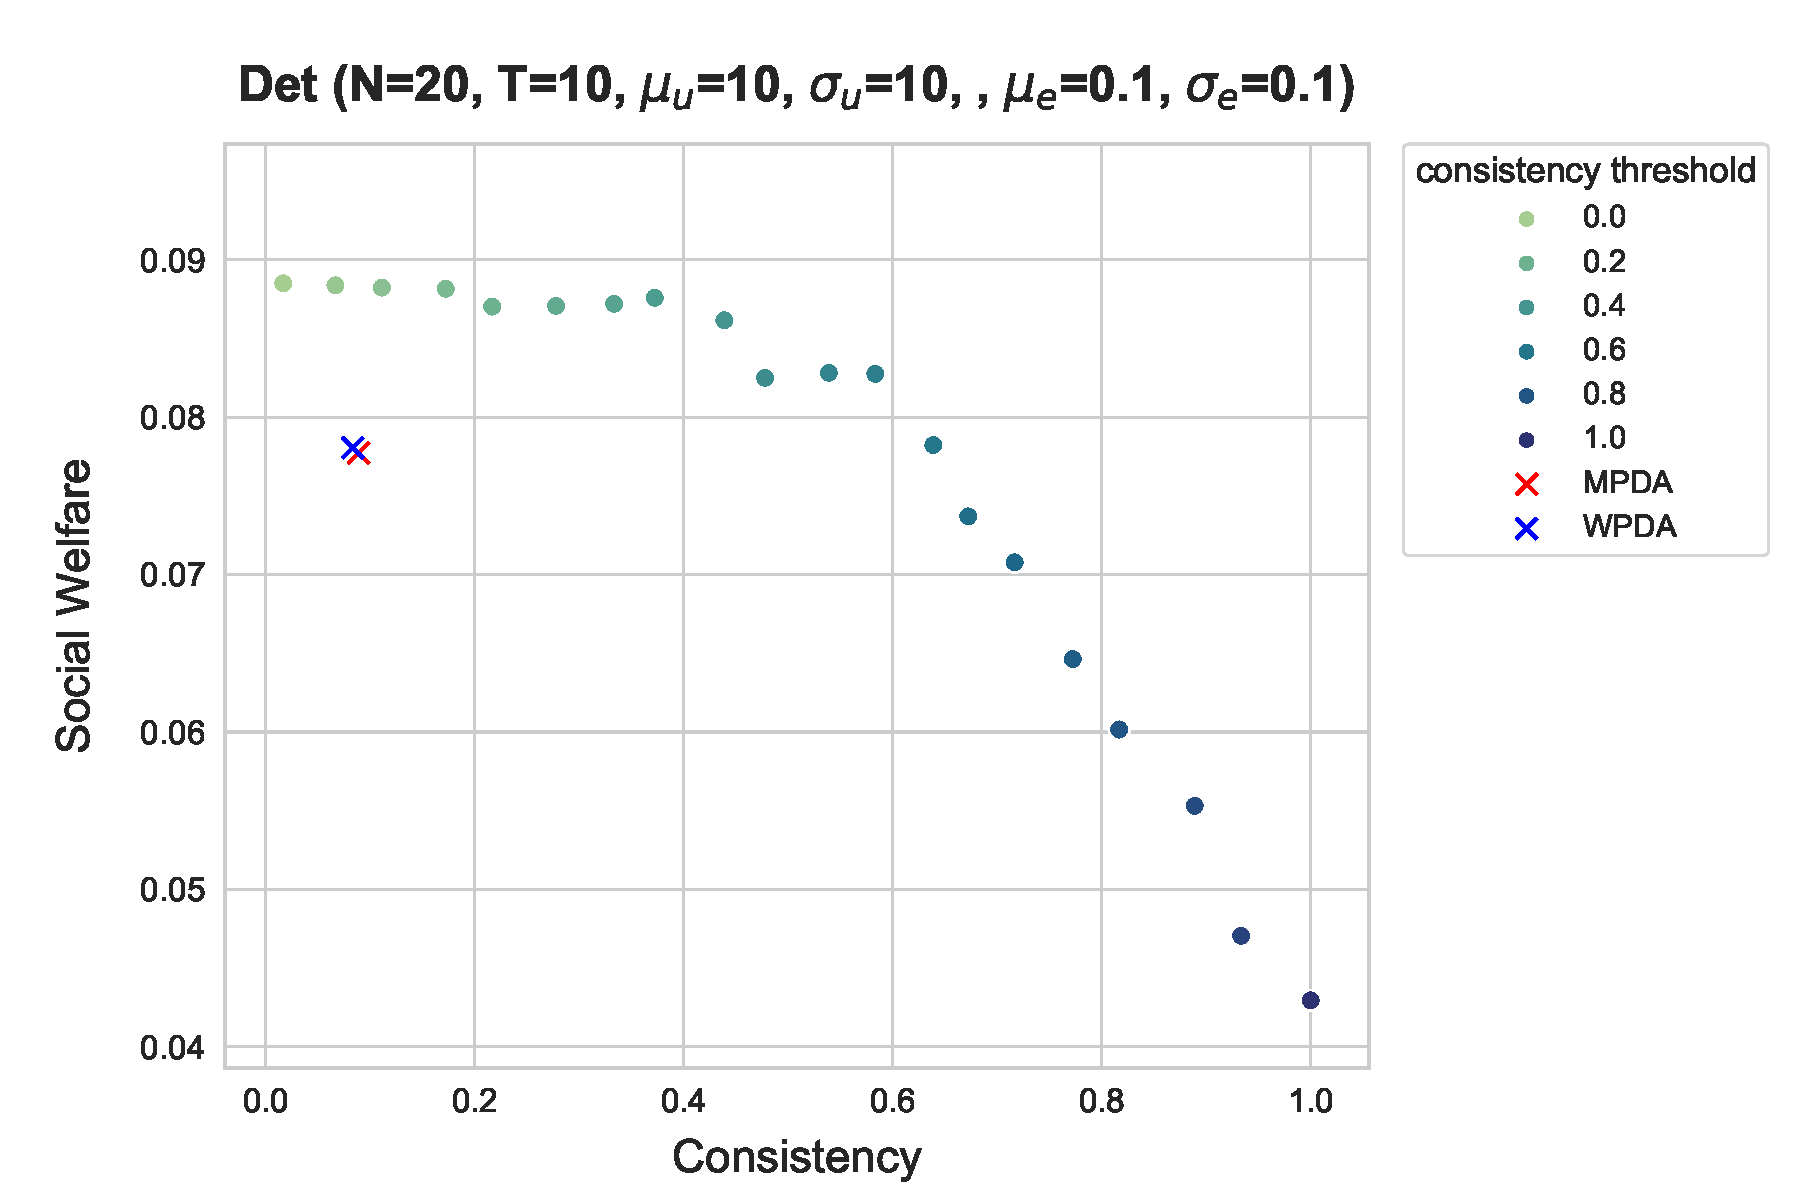
\includegraphics[width=0.32\linewidth]{figures/algs/Det_20_10_10_10.pdf}
    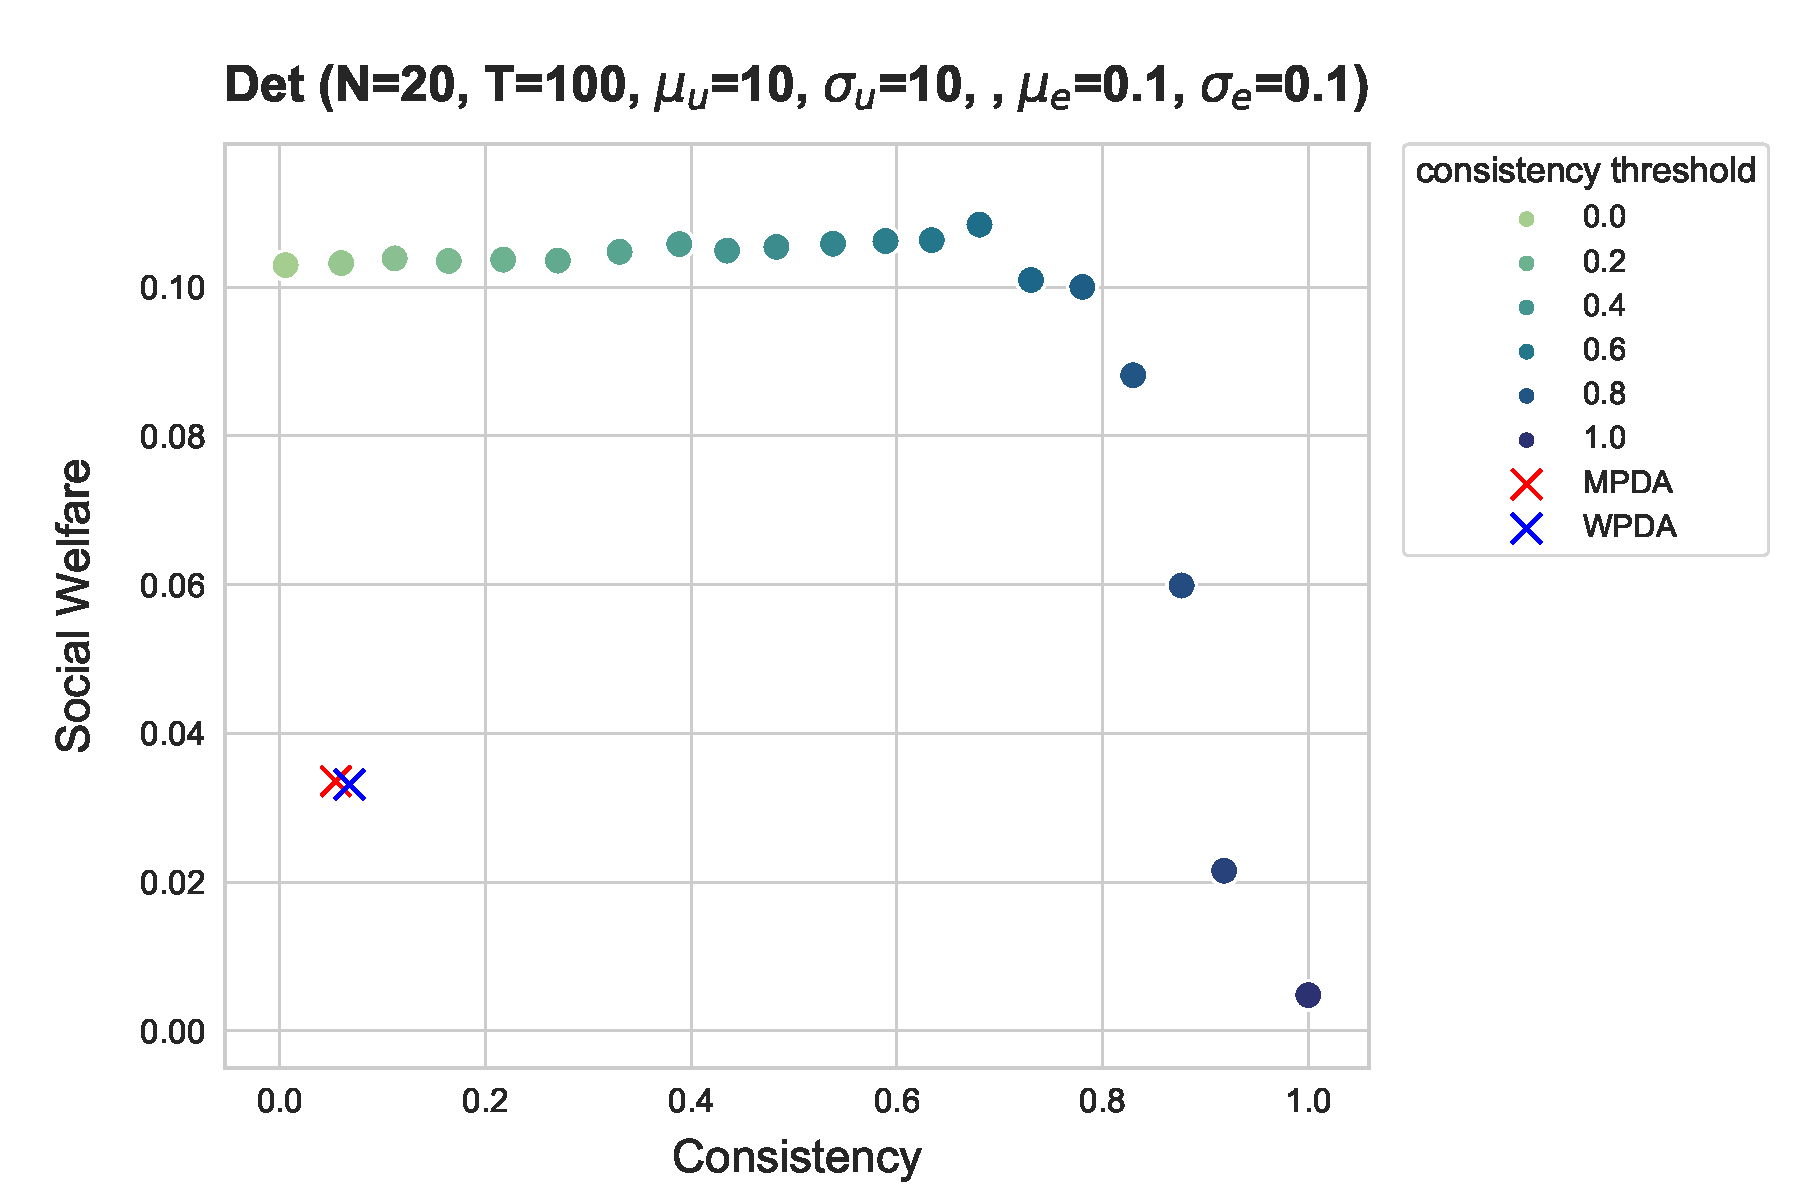
\includegraphics[width=0.32\linewidth]{figures/algs/Det_20_100_10_10.pdf}
    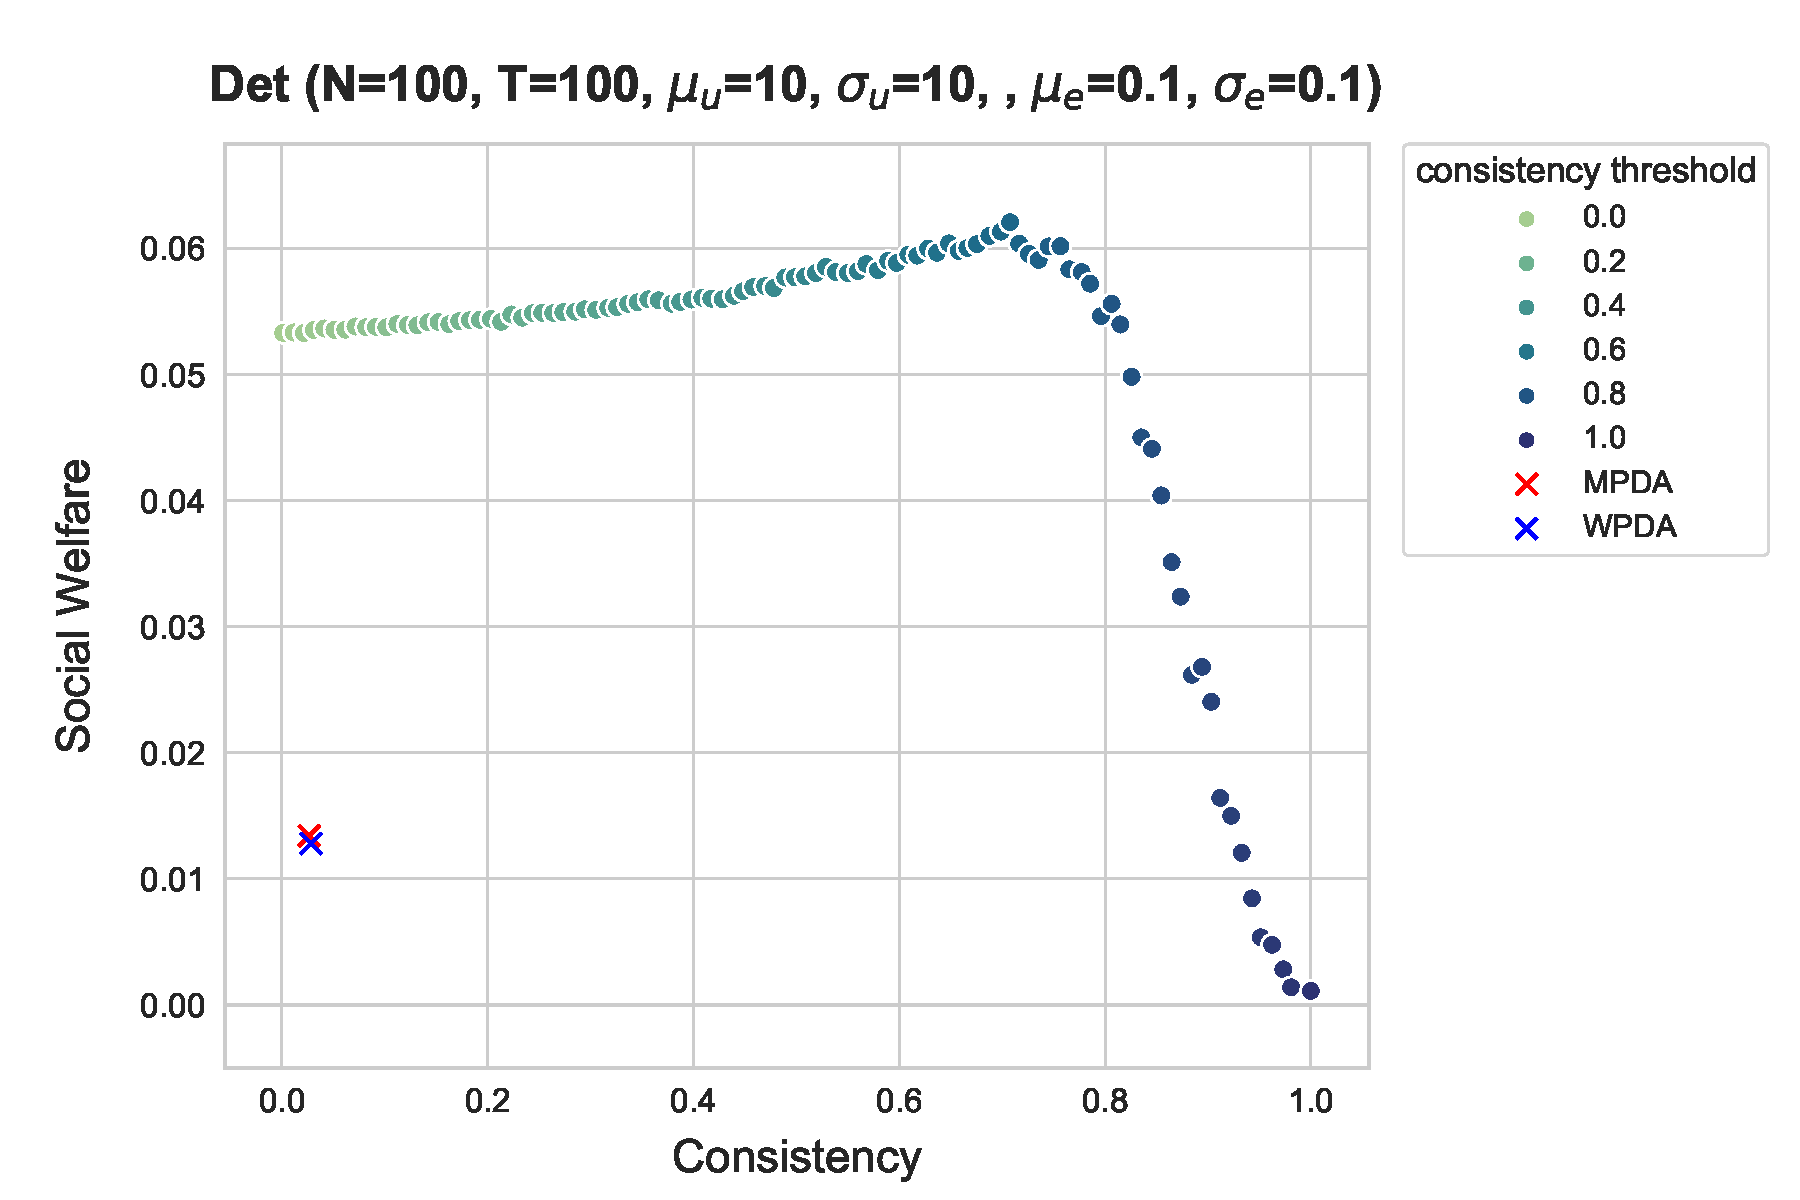
\includegraphics[width=0.32\linewidth]{figures/algs/Det_100_100_10_10.pdf}
    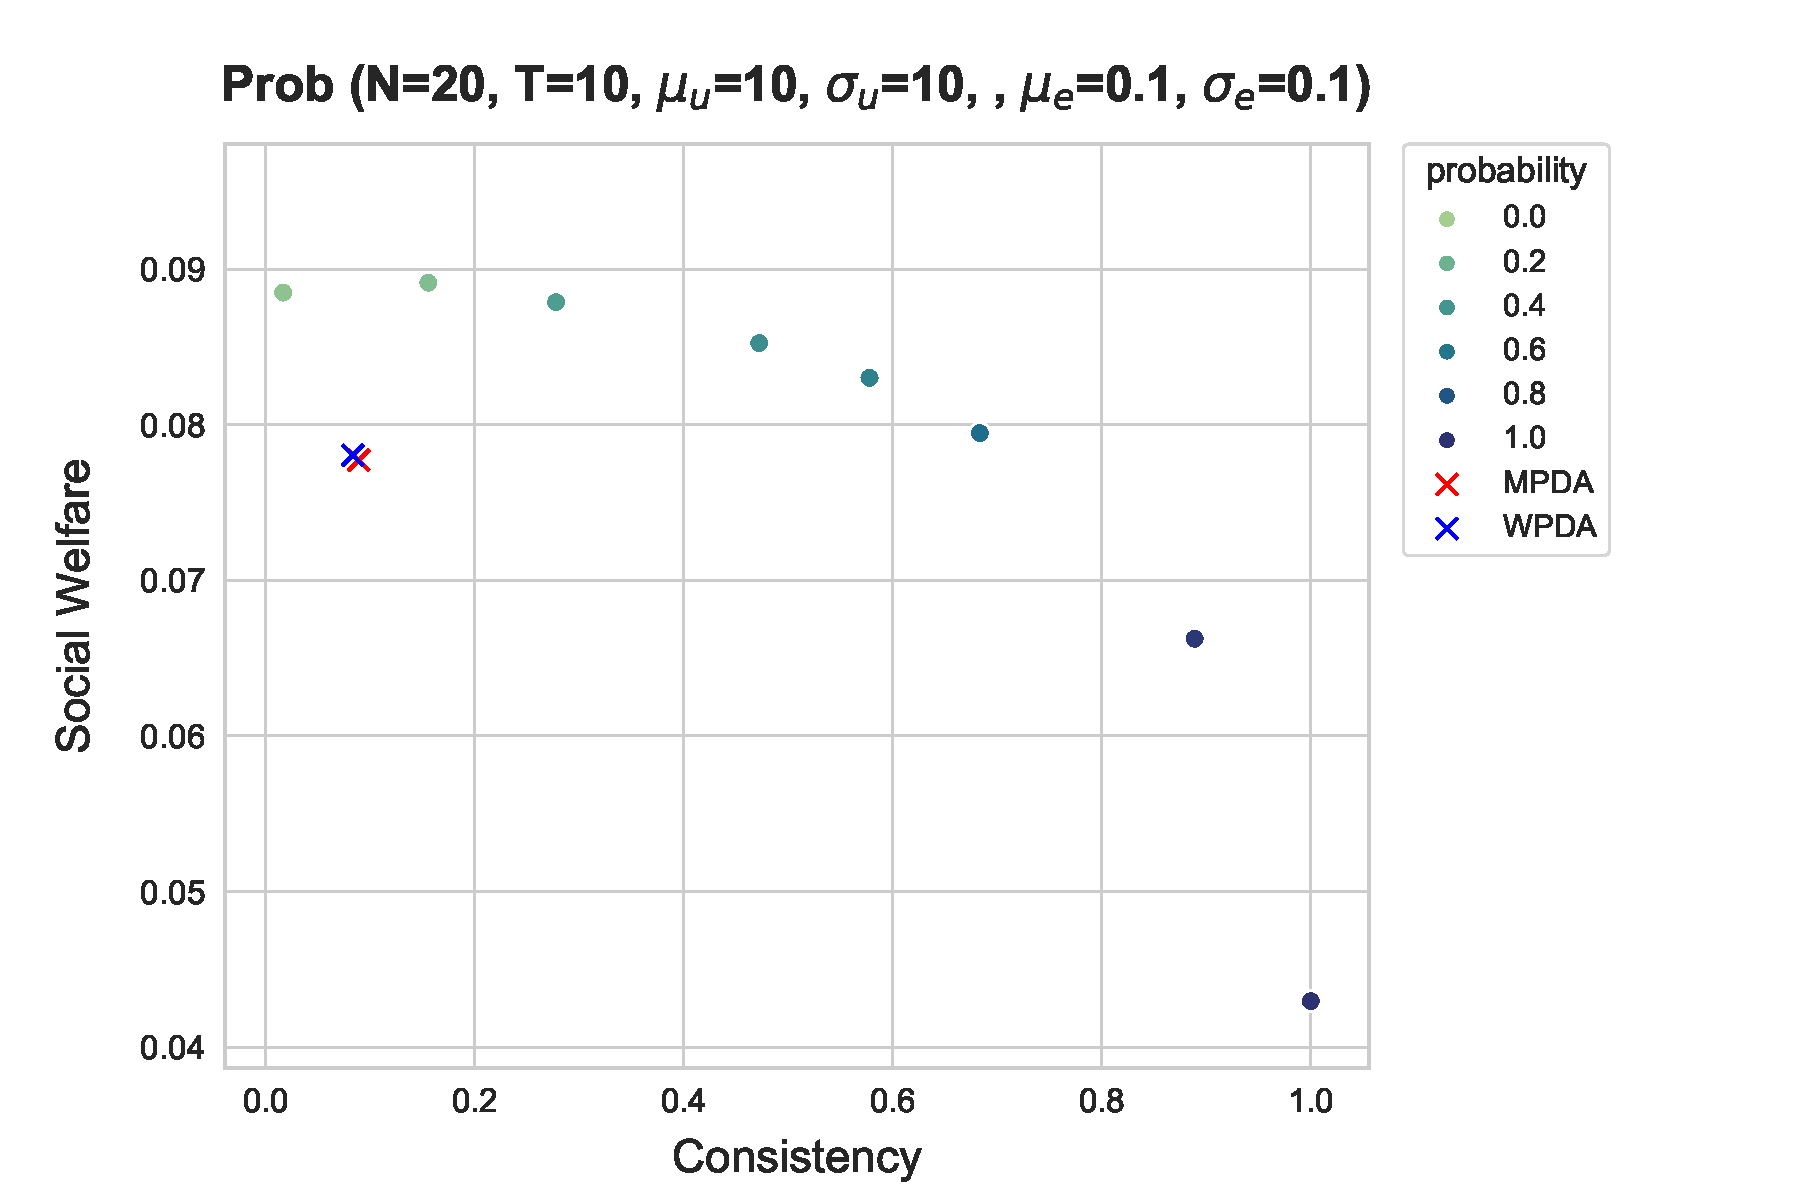
\includegraphics[width=0.32\linewidth]{figures/algs/Prob_20_10_10_10.pdf}
    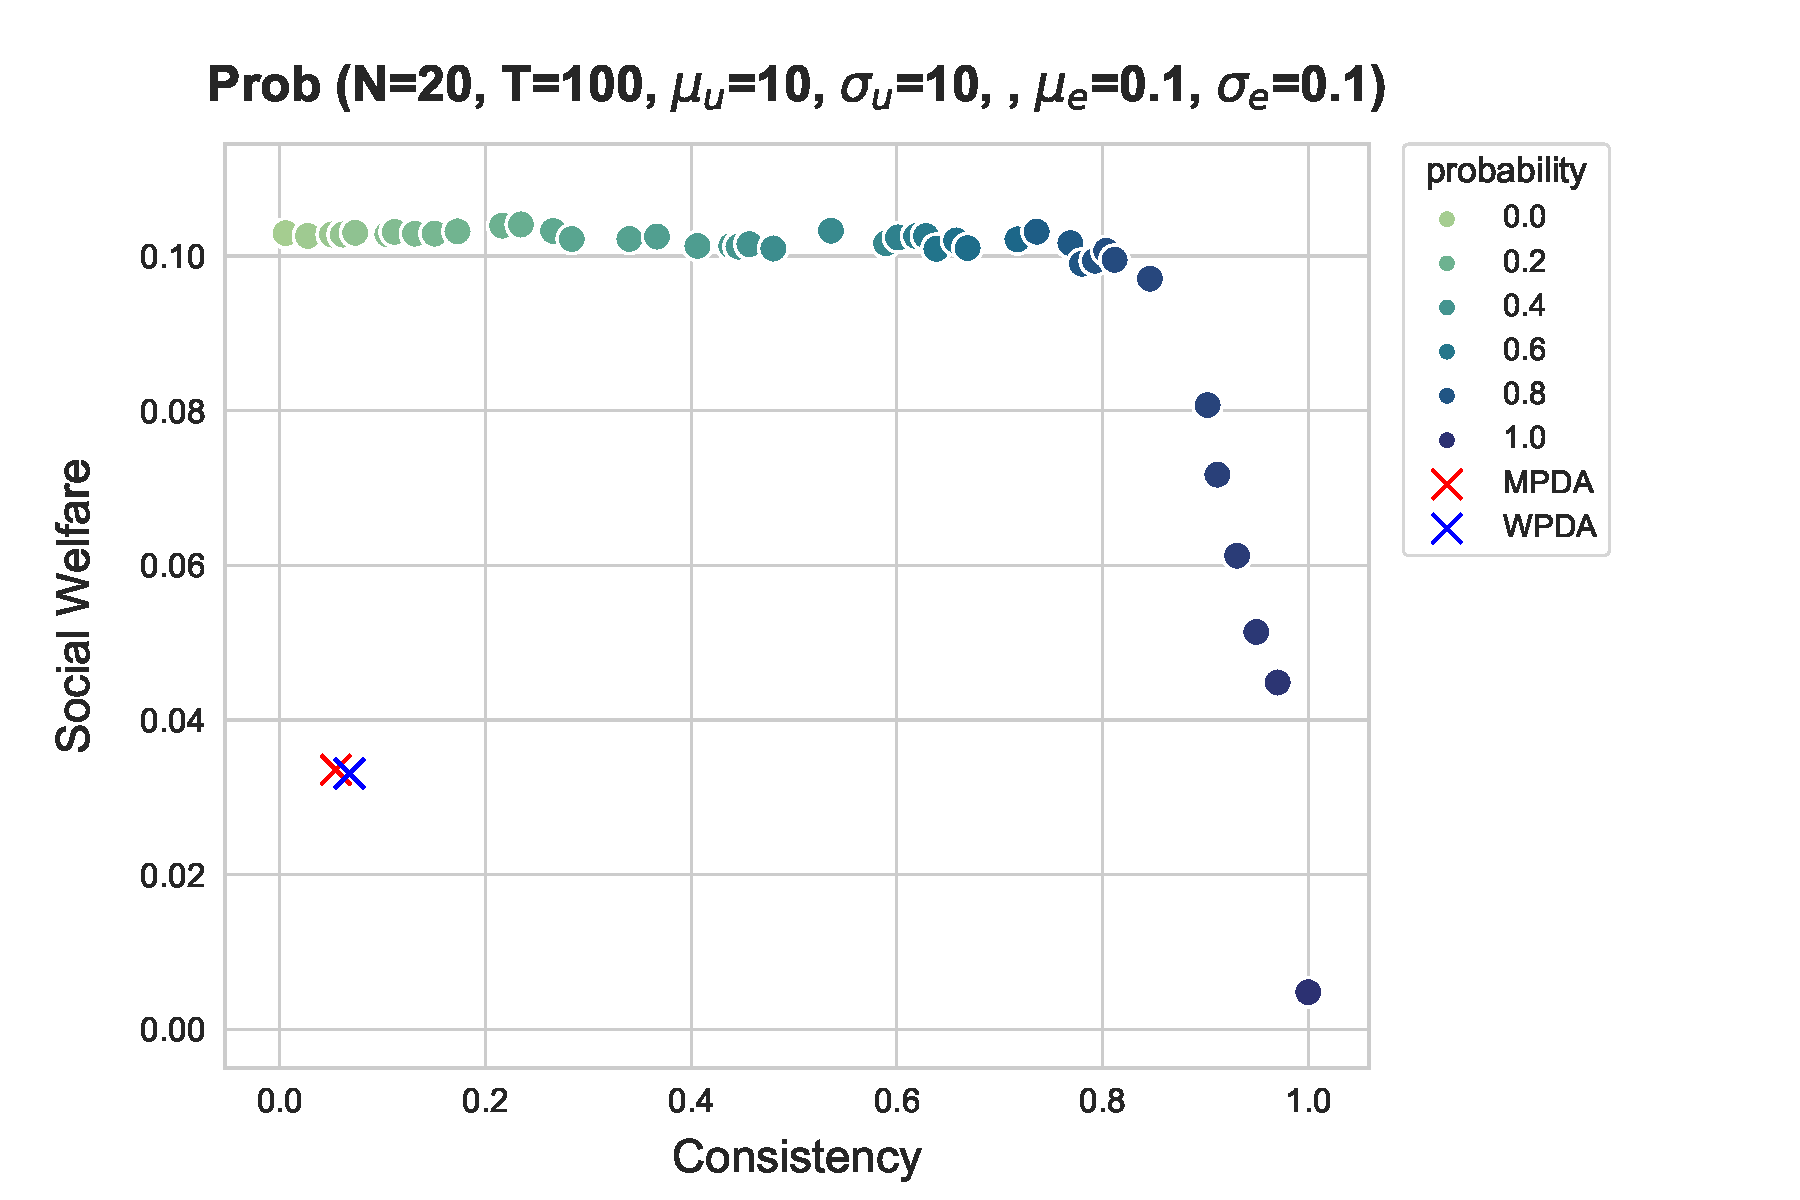
\includegraphics[width=0.32\linewidth]{figures/algs/Prob_20_100_10_10.pdf}
    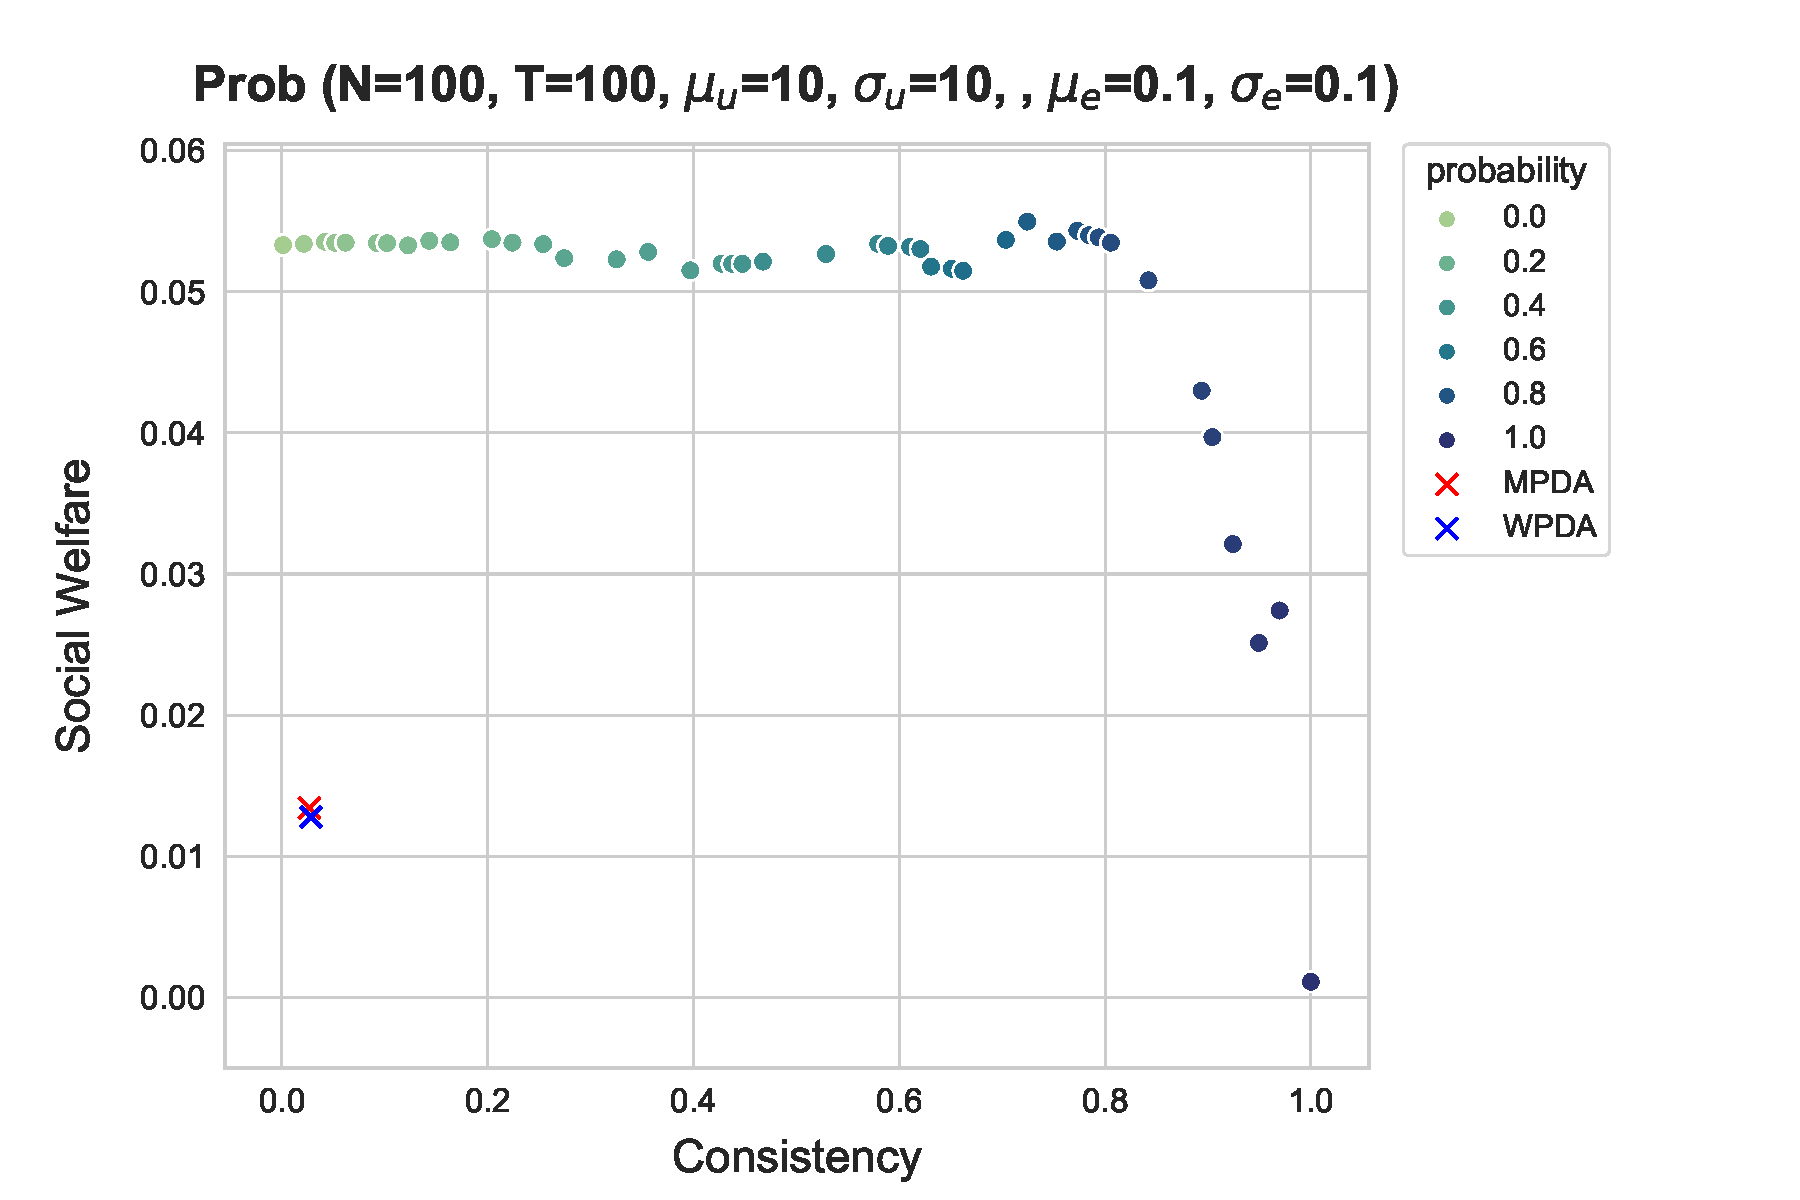
\includegraphics[width=0.32\linewidth]{figures/algs/Prob_100_100_10_10.pdf}
    \caption{Det (top row) and Prob (bottom row) algorithms in the setting where utilities are initialized with $\mathcal{N}(10, 10^2)$ and excitements are initialized with $\mathcal{N}(0.1, 0.1^2)$, with 20 agents and 10 time steps (left column), 20 agents and 100 time steps (middle column), and 100 agents and 100 time steps (right column) respectively.}
    \label{fig:algs}
\end{figure}
\begin{wrapfigure}{R}{0.3\textwidth}
     \vspace{-7mm}
        \centering
        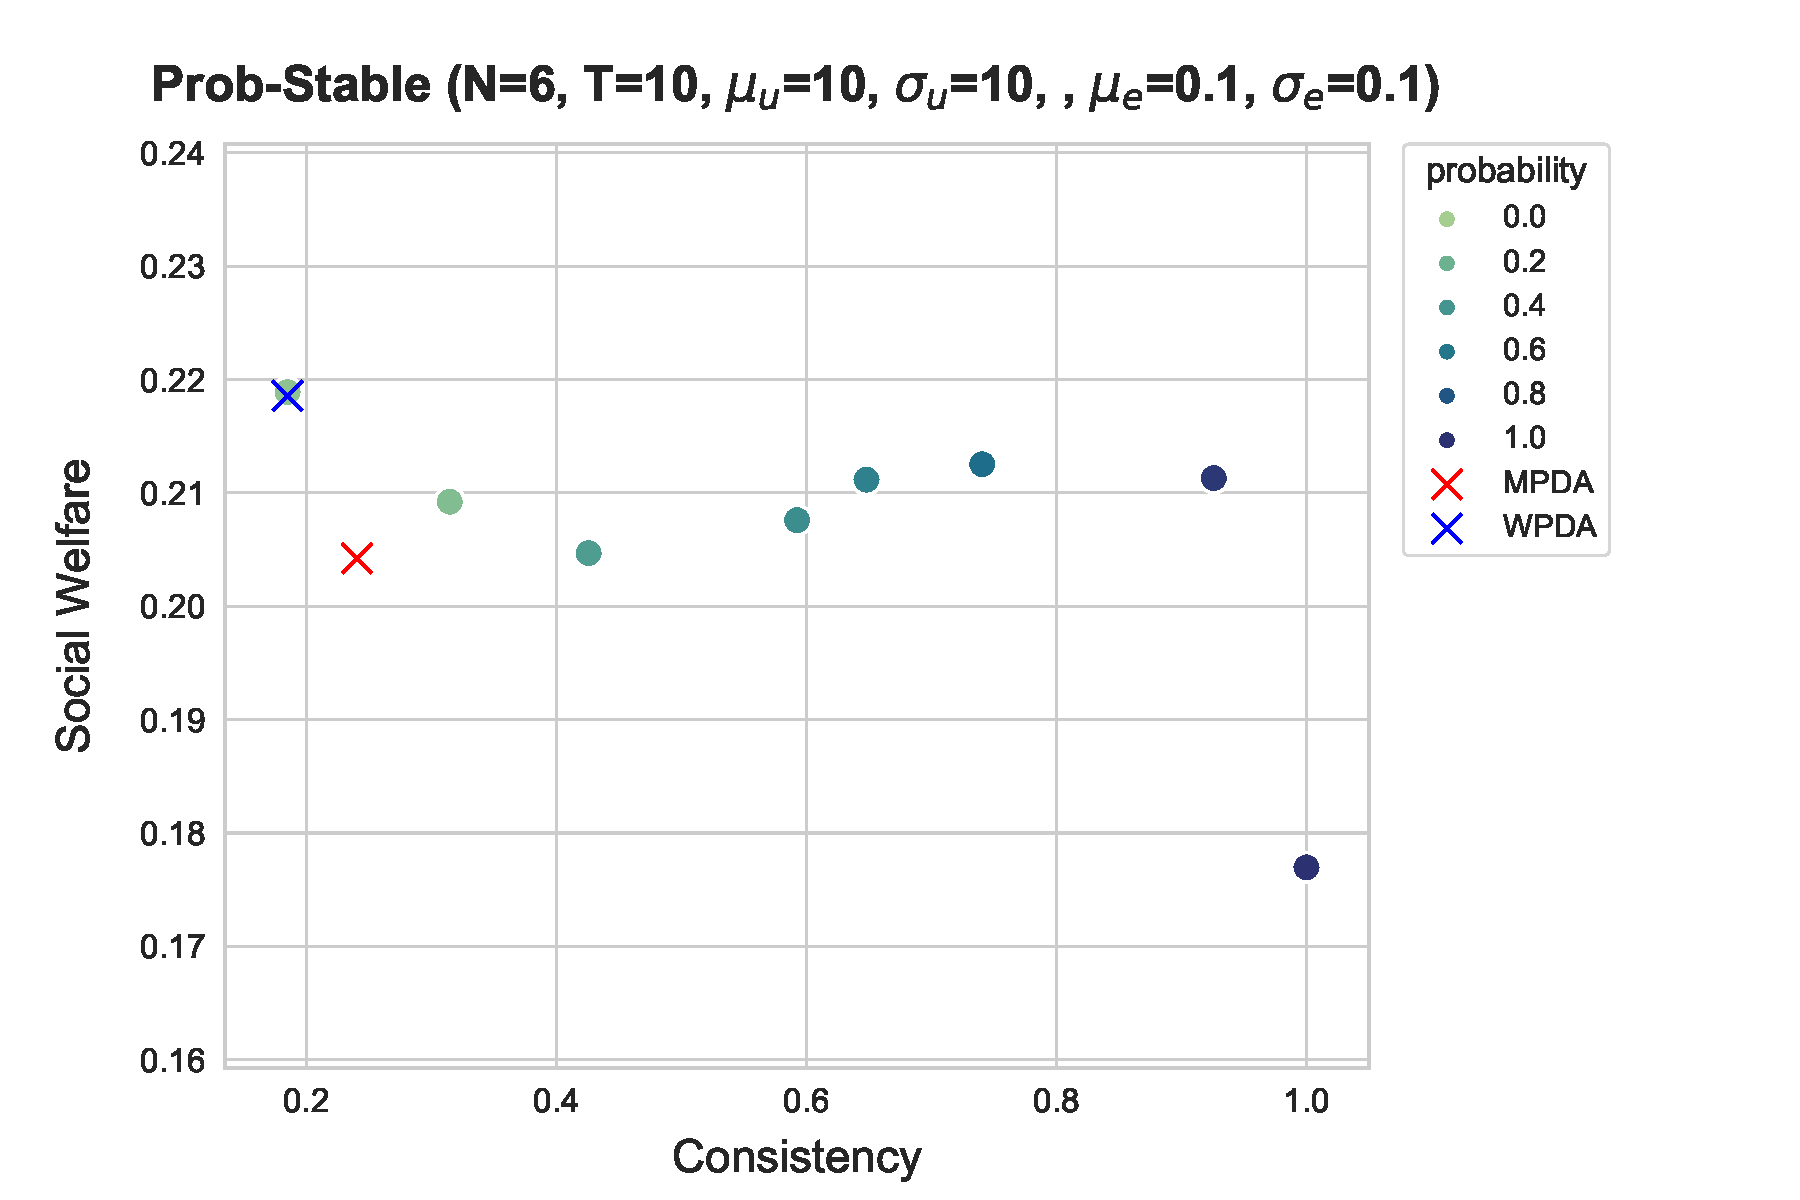
\includegraphics[width=0.3\textwidth]{figures/algs/Prob-Stable_6_10_10_10.pdf}
        \caption{Prob-Stable for $N=6$ and $T=10$.
        \label{fig:prob-stable}}
     \vspace{-15mm}
\end{wrapfigure}

\paragraph{Algorithms} We next run MPDA, WPDA, Det, Prob and Prob-Stable in the dynamics setting with $\mu_u = \sigma_u = 10$ and $\mu_e = \sigma_e = 0.1$. We choose this setting since the initialized utilities are diverse and the excitements are not too drastic. We experiment with $(N=20, T=10)$, $(N=20, T=100)$ and $(N=100, T=100)$ respectively. Fig.~\ref{fig:algs} showcases the results of Det and Prob compared to MPDA and WPDA. For both Det and Prob, we see that a higher threshold of $c$ or $p$, which constrains the results to have a higher consistency, generally leads to smaller social welfare. Nevertheless, we observe that with $T=100$ total time steps, the social welfare peaks at around 0.6 consistency, which shows that putting a constraint on the marriage consistency leads to better long-term average social welfare than allowing agents to marry greedily according to their utilities at every time step. Furthermore, we show that with more agents and longer time horizon, the performance gap between MPDA/WPDA and Det/Prob increases in terms of both consistency and social welfare. This is likely due to the fact that with more agents and more time steps, it is harder for a matching to stay stable and achieve maximum social welfare. A perhaps more fair comparison is shown in Fig.~\ref{fig:prob-stable} with the Prob-Stable algorithm, where WPDA has a closer performance as Prob-Stable with $p=0$.

\begin{figure}
    \centering
    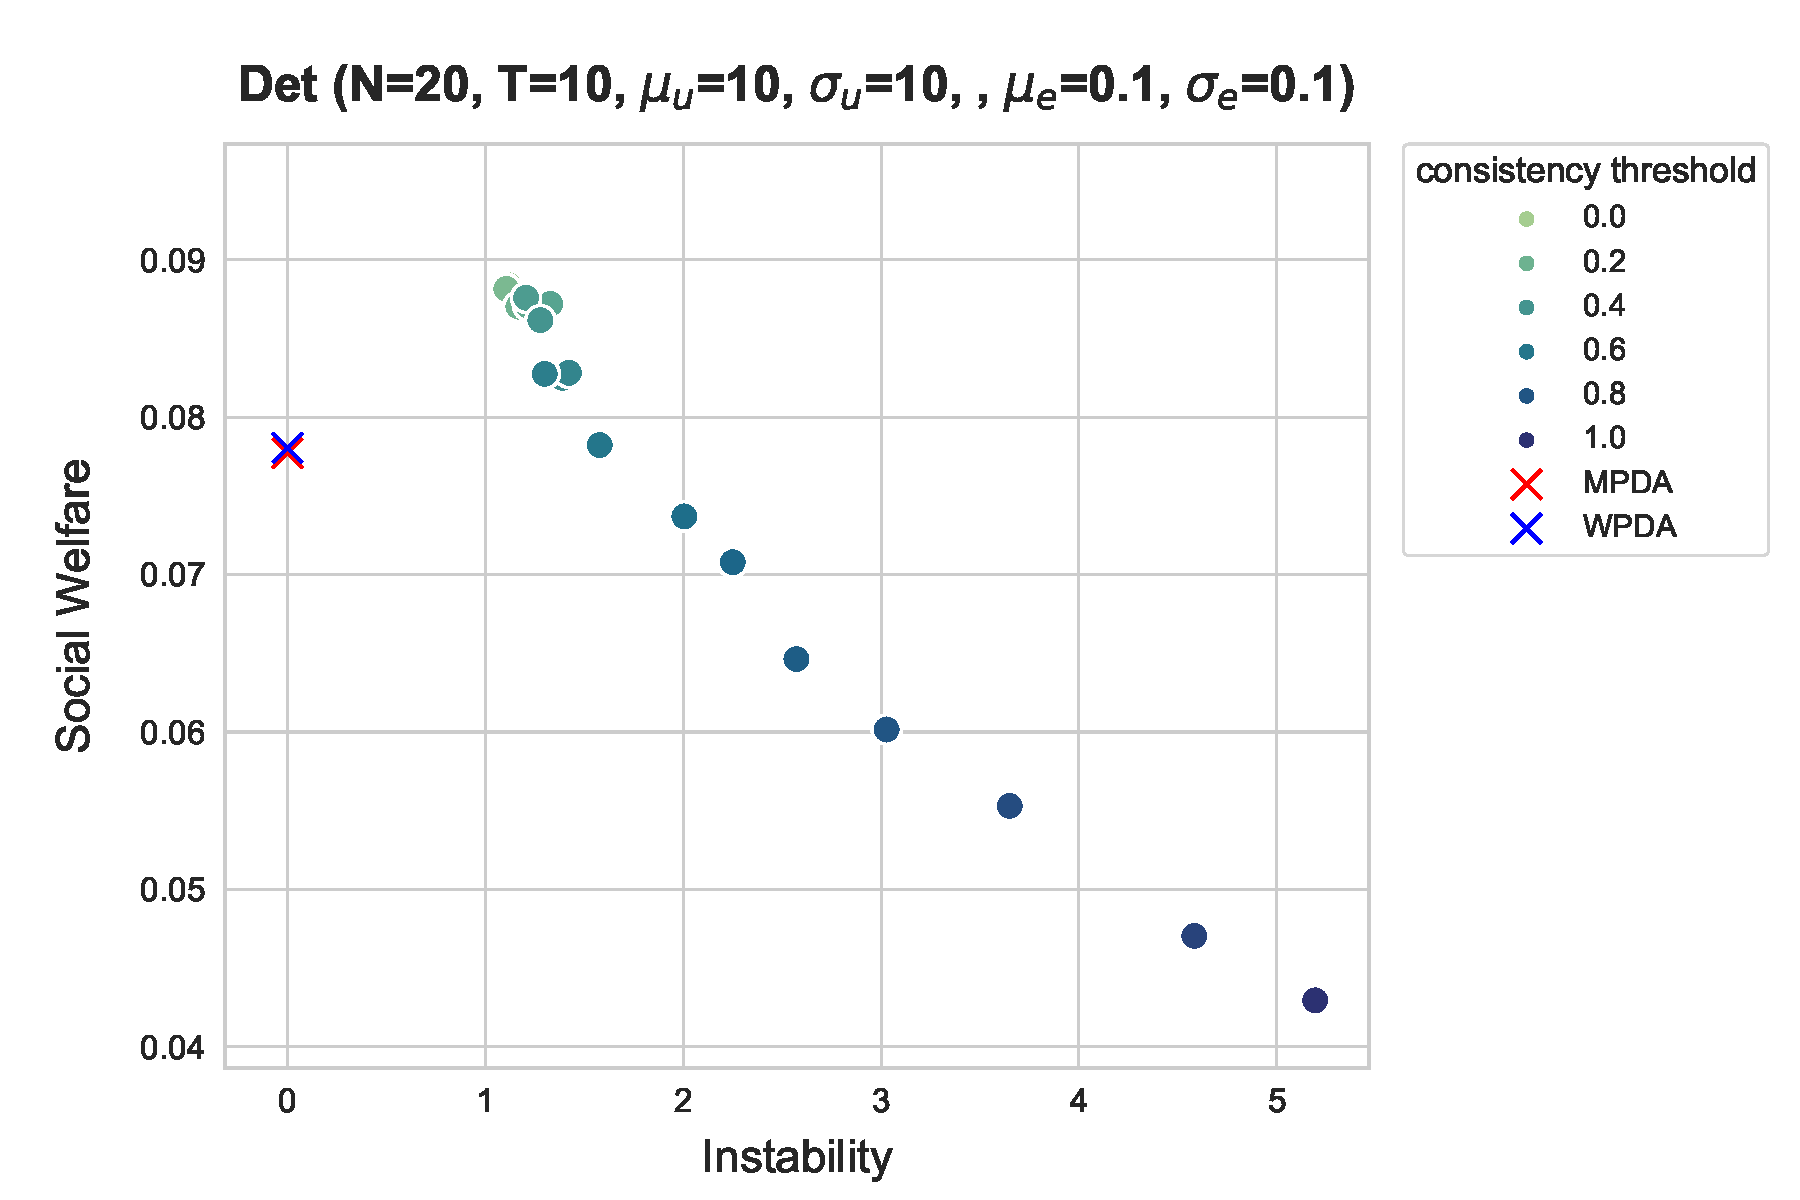
\includegraphics[width=0.32\linewidth]{figures/algs/Det_sw_20_10_10_10.pdf}
    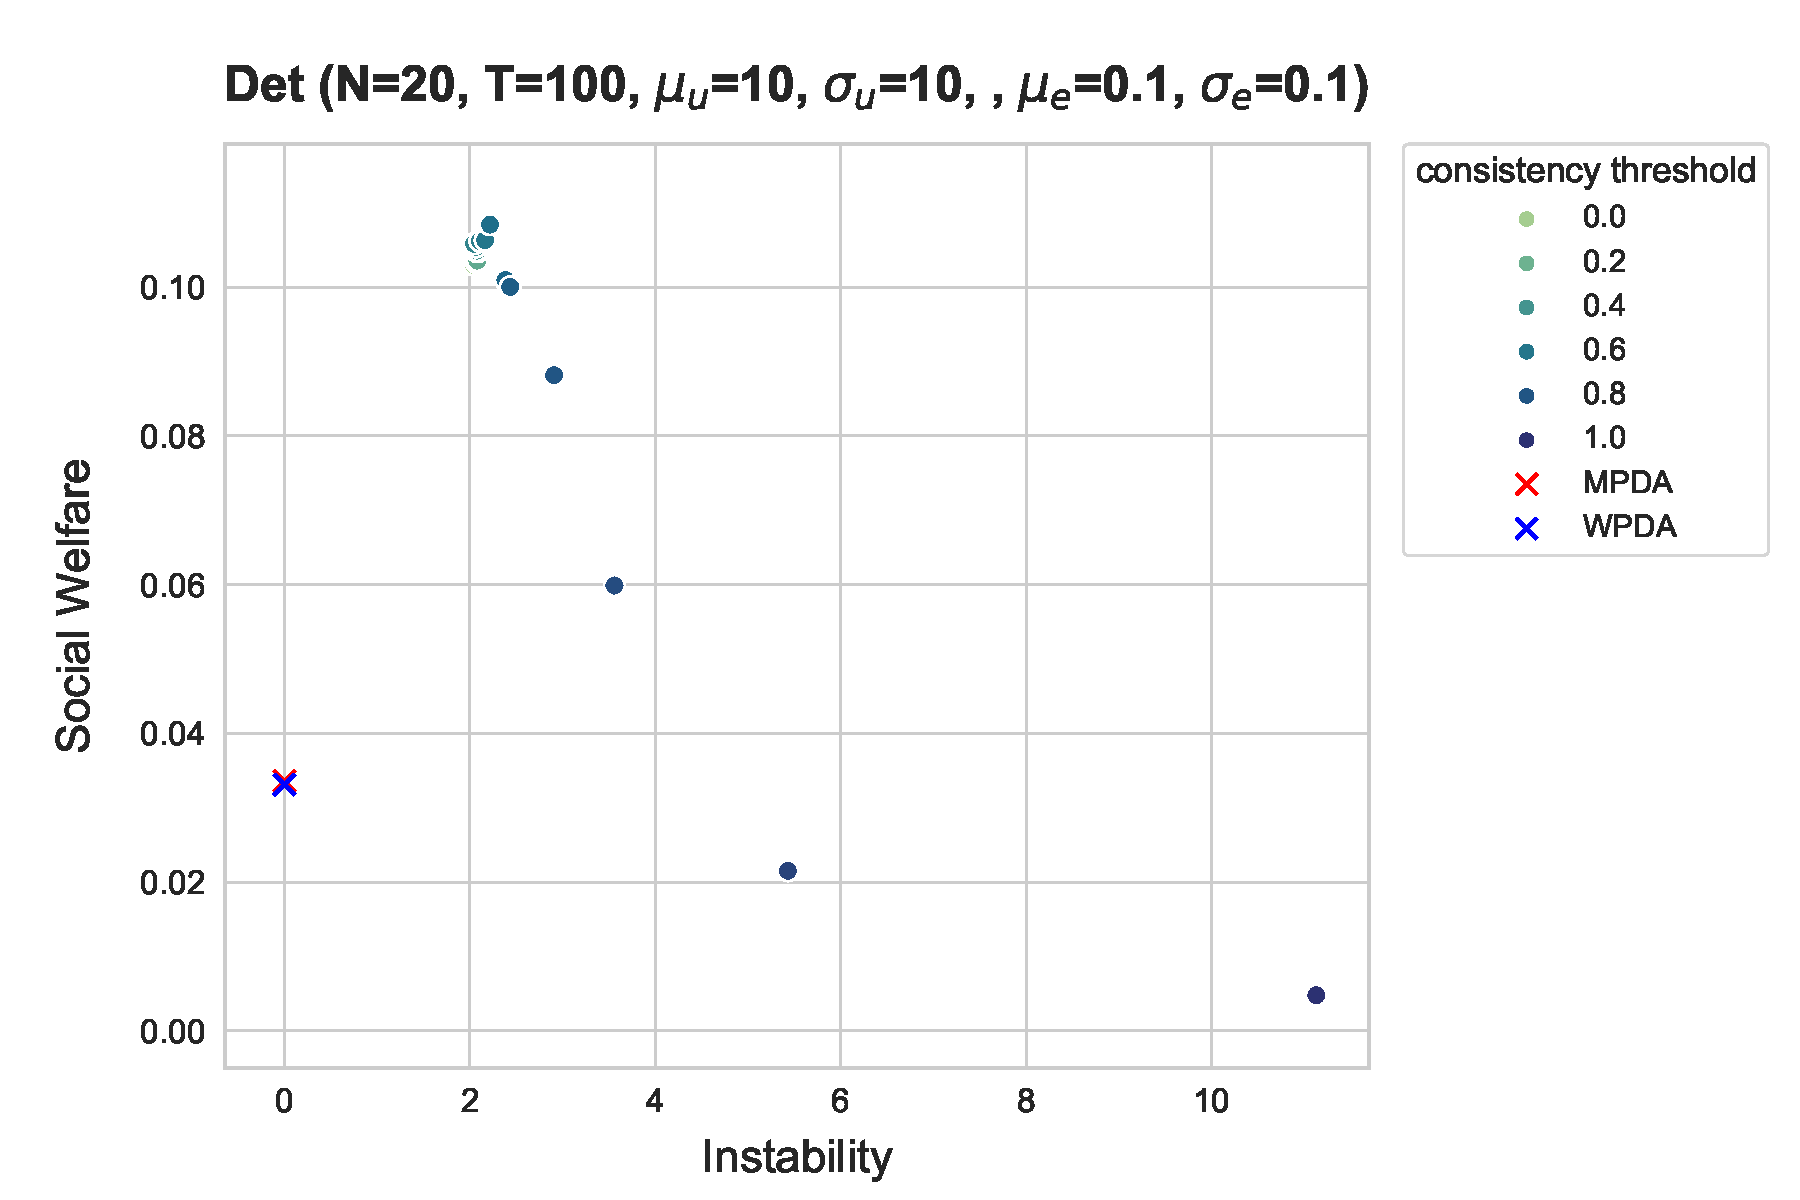
\includegraphics[width=0.32\linewidth]{figures/algs/Det_sw_20_100_10_10.pdf}
    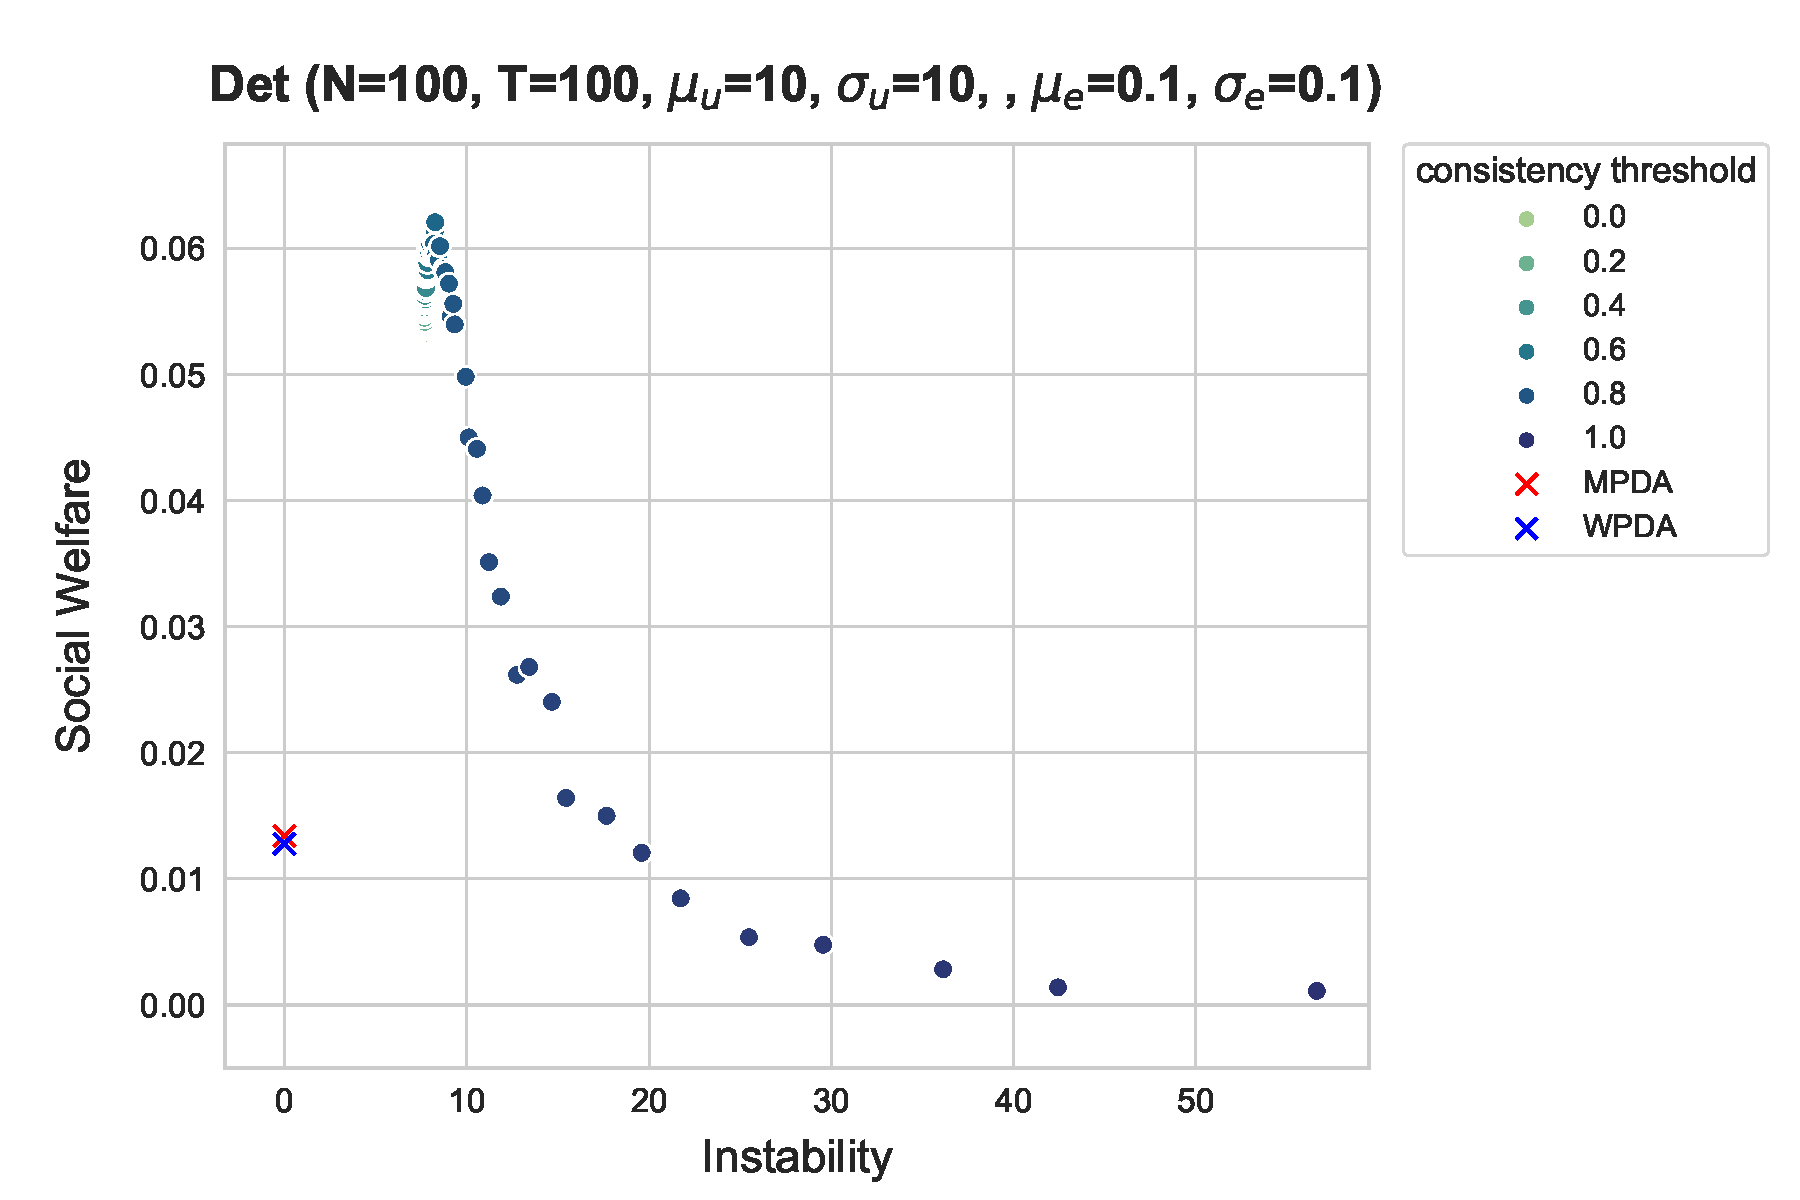
\includegraphics[width=0.32\linewidth]{figures/algs/Det_sw_100_100_10_10.pdf}
    \caption{Instability vs. social welfare for Det vs. MPDA vs. WPDA, with 20 men/women and 10 time steps (left), 20 men/women and 100 time steps (middle), and 100 men/women and 100 time steps (right).}
    \label{fig:det-stability}
\end{figure}
\paragraph{Stability vs. Social Welfare} We also evaluate the stability of Det. Fig.~\ref{fig:det-stability} shows that high social welfare is generally correlated with low instability. However, matching with maximum social welfare is still unstable, and a stable matching can have a much lower social welfare compared to the maximum.
% 0.5 - 1 page
% Figures and analysis
% \begin{itemize}
%     \item Evaluation of the algorithms (trade-off plot)
%     \begin{itemize}
%         \item scatter plot for the algorithm family
%         \item variance plot for the algorithm family
%     \end{itemize}
%     \item Evaluation with various dynamics
%     \begin{itemize}
%         \item Plot the trade off curve with MPDA and update with match
%     \end{itemize}
% \end{itemize}

\section{Discussion}
In this work we introduce the dynamic stable matching setting where each agent's preference profile is associated with an underlying numerical utilities vector, which is subject to change over time. Hence, a good matching algorithm needs to produce matching that respects both social welfare and the longevity of marriages over time. Our empirical evaluations show that the classical stable matching algorithms produce very inconsistent matching that also does not have high social welfare in settings with more agents and longer time horizon, compared to a few other matching algorithms. Because current matching algorithms have no acknoledgement of horizon, it is expected for them exhibit such behaviour. In future work, it would interesting to investigate methododlogies that are aware of the dynamics of agents and could control stability and optimality over longer horizons. Such methods are much more useful for everyday settings as real environments exhbits complex but sometimes characterizable dynamics. Further, in this work we considered simulated dynamics using faily basic Gaussian distributions, thus is would be further interesting to consider more realistic dynamics based on statistics say.


\bibliographystyle{abbrv}
\bibliography{ref}

\end{document}
% 
